% uWaterloo Thesis Template for LaTeX 
% Last Updated May 24, 2011 by Stephen Carr, IST Client Services
% FOR ASSISTANCE, please send mail to rt-IST-CSmathsci@ist.uwaterloo.ca

% Effective October 2006, the University of Waterloo 
% requires electronic thesis submission. See the uWaterloo thesis regulations at
% http://www.grad.uwaterloo.ca/Thesis_Regs/thesistofc.asp.

% DON'T FORGET TO ADD YOUR OWN NAME AND TITLE in the "hyperref" package
% configuration below. THIS INFORMATION GETS EMBEDDED IN THE PDF FINAL PDF DOCUMENT.
% You can view the information if you view Properties of the PDF document.

% Many faculties/departments also require one or more printed
% copies. This template attempts to satisfy both types of output. 
% It is based on the standard "book" document class which provides all necessary 
% sectioning structures and allows multi-part theses.

% DISCLAIMER
% To the best of our knowledge, this template satisfies the current uWaterloo requirements.
% However, it is your responsibility to assure that you have met all 
% requirements of the University and your particular department.
% Many thanks to the feedback from many graduates that assisted the development of this template.

% -----------------------------------------------------------------------

% By default, output is produced that is geared toward generating a PDF 
% version optimized for viewing on an electronic display, including 
% hyperlinks within the PDF.
 
% E.g. to process a thesis called "mythesis.tex" based on this template, run:

% pdflatex mythesis	-- first pass of the pdflatex processor
% bibtex mythesis	-- generates bibliography from .bib data file(s) 
% pdflatex mythesis	-- fixes cross-references, bibliographic references, etc
% pdflatex mythesis	-- fixes cross-references, bibliographic references, etc

% If you use the recommended LaTeX editor, Texmaker, you would open the mythesis.tex
% file, then click the pdflatex button. Then run BibTeX (under the Tools menu).
% Then click the pdflatex button two more times. If you have an index as well,
% you'll need to run MakeIndex from the Tools menu as well, before running pdflatex
% the last two times.

% N.B. The "pdftex" program allows graphics in the following formats to be
% included with the "\includegraphics" command: PNG, PDF, JPEG, TIFF
% Tip 1: Generate your figures and photos in the size you want them to appear
% in your thesis, rather than scaling them with \includegraphics options.
% Tip 2: Any drawings you do should be in scalable vector graphic formats:
% SVG, PNG, WMF, EPS and then converted to PNG or PDF, so they are scalable in
% the final PDF as well.
% Tip 3: Photographs should be cropped and compressed so as not to be too large.

% To create a PDF output that is optimized for double-sided printing: 
%
% 1) comment-out the \documentclass statement in the preamble below, and
% un-comment the second \documentclass line.
%
% 2) change the value assigned below to the boolean variable
% "PrintVersion" from "false" to "true".

% --------------------- Start of Document Preamble -----------------------

% Specify the document class, default style attributes, and page dimensions
% For hyperlinked PDF, suitable for viewing on a computer, use this:
\documentclass[letterpaper,12pt,titlepage,oneside,final]{book}
 
% For PDF, suitable for double-sided printing, change the PrintVersion variable below
% to "true" and use this \documentclass line instead of the one above:
%\documentclass[letterpaper,12pt,titlepage,openright,twoside,final]{book}

% Some LaTeX commands I define for my own nomenclature.
% If you have to, it's better to change nomenclature once here than in a 
% million places throughout your thesis!
\newcommand{\package}[1]{\textbf{#1}} % package names in bold text
\newcommand{\cmmd}[1]{\textbackslash\texttt{#1}} % command name in tt font 
\newcommand{\href}[1]{#1} % does nothing, but defines the command so the
    % print-optimized version will ignore \href tags (redefined by hyperref pkg).
%\newcommand{\texorpdfstring}[2]{#1} % does nothing, but defines the command
% Anything defined here may be redefined by packages added below...

% This package allows if-then-else control structures.
\usepackage{ifthen}
\newboolean{PrintVersion}
\setboolean{PrintVersion}{false} 
% CHANGE THIS VALUE TO "true" as necessary, to improve printed results for hard copies
% by overriding some options of the hyperref package below.

%\usepackage{nomencl} % For a nomenclature (optional; available from ctan.org)
\usepackage{amsmath,amssymb,amstext} % Lots of math symbols and environments
\usepackage[pdftex]{graphicx} % For including graphics N.B. pdftex graphics driver 

% Hyperlinks make it very easy to navigate an electronic document.
% In addition, this is where you should specify the thesis title
% and author as they appear in the properties of the PDF document.
% Use the "hyperref" package 
% N.B. HYPERREF MUST BE THE LAST PACKAGE LOADED; ADD ADDITIONAL PKGS ABOVE
\usepackage[pdftex,letterpaper=true,pagebackref=false]{hyperref} % with basic options
		% N.B. pagebackref=true provides links back from the References to the body text. This can cause trouble for printing.
\hypersetup{
    plainpages=false,       % needed if Roman numbers in frontpages
    pdfpagelabels=true,     % adds page number as label in Acrobat's page count
    bookmarks=true,         % show bookmarks bar?
    unicode=false,          % non-Latin characters in Acrobat’s bookmarks
    pdftoolbar=true,        % show Acrobat’s toolbar?
    pdfmenubar=true,        % show Acrobat’s menu?
    pdffitwindow=false,     % window fit to page when opened
    pdfstartview={FitH},    % fits the width of the page to the window
    pdftitle={Efficient Temporal Synopsis of Social Media Streams},    % title: CHANGE THIS TEXT!
    pdfauthor={Younes Abouelnagah},    % author: CHANGE THIS TEXT! and uncomment this line
%    pdfsubject={Subject},  % subject: CHANGE THIS TEXT! and uncomment this line
%    pdfkeywords={keyword1} {key2} {key3}, % list of keywords, and uncomment this line if desired
    pdfnewwindow=true,      % links in new window
    colorlinks=true,        % false: boxed links; true: colored links
    linkcolor=blue,         % color of internal links
    citecolor=green,        % color of links to bibliography
    filecolor=magenta,      % color of file links
    urlcolor=cyan           % color of external links
}
\ifthenelse{\boolean{PrintVersion}}{   % for improved print quality, change some hyperref options
\hypersetup{	% override some previously defined hyperref options
%    colorlinks,%
    citecolor=black,%
    filecolor=black,%
    linkcolor=black,%
    urlcolor=black}
}{} % end of ifthenelse (no else)

% Setting up the page margins...
% uWaterloo thesis requirements specify a minimum of 1 inch (72pt) margin at the
% top, bottom, and outside page edges and a 1.125 in. (81pt) gutter
% margin (on binding side). While this is not an issue for electronic
% viewing, a PDF may be printed, and so we have the same page layout for
% both printed and electronic versions, we leave the gutter margin in.
% Set margins to minimum permitted by uWaterloo thesis regulations:
\setlength{\marginparwidth}{0pt} % width of margin notes
% N.B. If margin notes are used, you must adjust \textwidth, \marginparwidth
% and \marginparsep so that the space left between the margin notes and page
% edge is less than 15 mm (0.6 in.)
\setlength{\marginparsep}{0pt} % width of space between body text and margin notes
\setlength{\evensidemargin}{0.125in} % Adds 1/8 in. to binding side of all 
% even-numbered pages when the "twoside" printing option is selected
\setlength{\oddsidemargin}{0.125in} % Adds 1/8 in. to the left of all pages
% when "oneside" printing is selected, and to the left of all odd-numbered
% pages when "twoside" printing is selected
\setlength{\textwidth}{6.375in} % assuming US letter paper (8.5 in. x 11 in.) and 
% side margins as above
\raggedbottom

% The following statement specifies the amount of space between
% paragraphs. Other reasonable specifications are \bigskipamount and \smallskipamount.
\setlength{\parskip}{\medskipamount}

% The following statement controls the line spacing.  The default
% spacing corresponds to good typographic conventions and only slight
% changes (e.g., perhaps "1.2"), if any, should be made.
\renewcommand{\baselinestretch}{1.2} % this is the default line space setting

% By default, each chapter will start on a recto (right-hand side)
% page.  We also force each section of the front pages to start on 
% a recto page by inserting \cleardoublepage commands.
% In many cases, this will require that the verso page be
% blank and, while it should be counted, a page number should not be
% printed.  The following statements ensure a page number is not
% printed on an otherwise blank verso page.
\let\origdoublepage\cleardoublepage
\newcommand{\clearemptydoublepage}{%
  \clearpage{\pagestyle{empty}\origdoublepage}}
\let\cleardoublepage\clearemptydoublepage

%======================================================================
%   L O G I C A L    D O C U M E N T -- the content of your thesis
%======================================================================

\usepackage[normalem]{ulem}

\usepackage{pdflscape}
\usepackage{mathtools}

\usepackage{algorithm2e}



\usepackage{multirow}

\begin{document}

% For a large document, it is a good idea to divide your thesis
% into several files, each one containing one chapter.
% To illustrate this idea, the "front pages" (i.e., title page,
% declaration, borrowers' page, abstract, acknowledgements,
% dedication, table of contents, list of tables, list of figures,
% nomenclature) are contained within the file "uw-ethesis-frontpgs.tex" which is
% included into the document by the following statement.
%----------------------------------------------------------------------
% FRONT MATERIAL
%----------------------------------------------------------------------
% T I T L E   P A G E
% -------------------
% Last updated May 24, 2011, by Stephen Carr, IST-Client Services
% The title page is counted as page `i' but we need to suppress the
% page number.  We also don't want any headers or footers.
\pagestyle{empty}
\pagenumbering{roman}

% The contents of the title page are specified in the "titlepage"
% environment.
\begin{titlepage}
        \begin{center}
        \vspace*{1.0cm}

        \Huge
        {\bf Efficient Temporal Synopsis of Social Media Streams }

        \vspace*{1.0cm}

        \normalsize
        by \\

        \vspace*{1.0cm}

        \Large
       Younes Abouelnagah\\

        \vspace*{3.0cm}

        \normalsize
        A thesis \\
        presented to the University of Waterloo \\ 
        in fulfillment of the \\
        thesis requirement for the degree of \\
        Master of Math \\
        in \\
        Computer Science \\

        \vspace*{2.0cm}

        Waterloo, Ontario, Canada, 2013 \\

        \vspace*{1.0cm}

        \copyright\ Younes Abouelnagah 2013 \\
        \end{center}
\end{titlepage}

% The rest of the front pages should contain no headers and be numbered using Roman numerals starting with `ii'
\pagestyle{plain}
\setcounter{page}{2}

\cleardoublepage % Ends the current page and causes all figures and tables that have so far appeared in the input to be printed.
% In a two-sided printing style, it also makes the next page a right-hand (odd-numbered) page, producing a blank page if necessary.
 


% D E C L A R A T I O N   P A G E
% -------------------------------
  % The following is the sample Delaration Page as provided by the GSO
  % December 13th, 2006.  It is designed for an electronic thesis.
  \noindent
I hereby declare that I am the sole author of this thesis. This is a true copy of the thesis, including any required final revisions, as accepted by my examiners.

  \bigskip
  
  \noindent
I understand that my thesis may be made electronically available to the public.

\cleardoublepage
%\newpage

% A B S T R A C T
% ---------------

\begin{center}\textbf{Abstract}\end{center}
Search and summarization of streaming social media, such as Twitter, requires the ongoing analysis of large volumes of data with dynamically changing characteristics.  Tweets are short and repetitious~--~lacking context and structure~--~making it difficult to generate a coherent synopsis of events within a given time period.  Although some established algorithms for frequent itemset analysis might provide an efficient foundation for synopsis generation, the unmodified application of standard methods produces a complex mass of rules, dominated by common language constructs and many trivial variations on topically related results.  Moreover, these results are not necessarily specific to events within the time period of interest.  To address these problems, we build upon the Linear time Closed itemset Mining (LCM) algorithm, which is particularly suited to the large and sparse vocabulary of tweets.  LCM generates only closed itemsets, providing an immediate reduction in the number of trivial results.  To reduce the impact of function words and common language constructs, we apply a filtering step that preserves these terms only when they may form part of a relevant collocation.  To further reduce trivial results, we propose a novel strengthening of the closure condition of LCM to retain only those results that exceed a threshold of distinctiveness.  Finally, we perform temporal ranking, based on information gain, to identify results that are particularly relevant to the time period of interest.  We evaluate our work over a collection of tweets gathered in late 2012, exploring the efficiency and filtering characteristic of each processing step, both individually and collectively.  Based on our experience, the resulting synopses from various time periods provide understandable and meaningful pictures of events within those periods, with potential application to tasks such as temporal summarization and query expansion for search.

\cleardoublepage
%\newpage

% A C K N O W L E D G E M E N T S
% -------------------------------

\begin{center}\textbf{Acknowledgements}\end{center}
I would like to thank all the people who made this possible.
First and foremost, my supervisor Charles Clarke for giving me
the opportunity to join such a great university,
and for providing a very encouraging learning environment.
Second, my family for making my life worry free, 
specially my wife Nada who was very patient 
during all the time I was away from her.
Last but not least, my colleagues in this journey of
development with whom I worked and grew.
 

\cleardoublepage
%\newpage

% D E D I C A T I O N
% -------------------

\begin{center}\textbf{Dedication}\end{center}

This is dedicated to the my people struggling for freedom and democracy in the Arab world, while I comfortably study in beautiful Canada.
\cleardoublepage
%\newpage

% T A B L E   O F   C O N T E N T S
% ---------------------------------
\renewcommand\contentsname{Table of Contents}
\tableofcontents
\cleardoublepage
\phantomsection
%\newpage

% L I S T   O F   T A B L E S
% ---------------------------
\addcontentsline{toc}{chapter}{List of Tables}
\listoftables
\cleardoublepage
\phantomsection		% allows hyperref to link to the correct page
%\newpage

% L I S T   O F   F I G U R E S
% -----------------------------
\addcontentsline{toc}{chapter}{List of Figures}
\listoffigures
\cleardoublepage
\phantomsection		% allows hyperref to link to the correct page
%\newpage

% L I S T   O F   S Y M B O L S
% -----------------------------
% To include a Nomenclature section
% \addcontentsline{toc}{chapter}{\textbf{Nomenclature}}
% \renewcommand{\nomname}{Nomenclature}
% \printglossary
% \cleardoublepage
% \phantomsection % allows hyperref to link to the correct page
% \newpage

% Change page numbering back to Arabic numerals
\pagenumbering{arabic}

 

%----------------------------------------------------------------------
% MAIN BODY
%----------------------------------------------------------------------
% Because this is a short document, and to reduce the number of files
% needed for this template, the chapters are not separate
% documents as suggested above, but you get the idea. If they were
% separate documents, they would each start with the \chapter command, i.e, 
% do not contain \documentclass or \begin{document} and \end{document} commands.
%======================================================================
\chapter{Introduction}
%======================================================================
%\category{H.4}{Information Systems Applications}{Miscellaneous}
%A category including the fourth, optional field follows...
%\category{D.2.8}{Software Engineering}{Metrics}[complexity measures, performance measures]

%\terms{Theory}

%\keywords{ACM proceedings, \LaTeX, text tagging}
\section{Social Media Text}
Text posted on social media outlets, such as Twitter, is a good and timely source of information
about real world events~\cite{ritter2012open}. 
It also includes posts about topics attracting the collective attention of user communities, 
such as Internet memes or large scale discussions~\cite{naaman2011hip}.
Nevertheless, the collective stream from all users is overwhelmed with personal
updates and non-informative chatter~\cite{java2007we,hurlock2011searching}. 
Furthermore, the attention span given to the majority of topics is quite short~\cite{kwak2010twitter}.
Timely finding posts about topics of interest requires an
efficient mining algorithm.

To realize the benefits of social media in giving a voice to ordinary people,
the algorithm should mine the content of posts 
without explicitly assigning weights based on merits of users. % to posts made by ``influencers''.
However, the nature of text in social media poses a challenge when applying
traditional text mining algorithms. 
Text in social media is usually short, undermining the effectiveness of within document frequency counting.
It lacks context, since posts are standalone and most platforms don't allow explicit linkage.
It also lacks structure and other useful formatting cues. 
One type of mining algorithms that can be applied to such data is frequent itemset mining.

\section{Frequent Itemset Mining}

Frequent itemset mining algorithms count the number of times each
combination of ``items'' appear together. 
This is called the support of the itemset.
An itemset is considered frequent if its support is above a threshold.
To mine textual data, an item can be a token and a set of items can
be considered as appearing together if they appear within the same document
or paragraph. The frequent itemset mining family of algorithms is fast and efficient,
however it is not readily suited for application on text. 
Following are a number of challenges faced when applying 
frequent itemset mining to textual data. In this thesis we address those problems, adapting frequent itemset mining to
social media text without degrading its efficiency:

\begin{enumerate}
\item
The number of itemsets mined grows with the number of
distinct items~--~which is particularly high in the text domain.
In social media, the problem is complicated by the continuous creation 
of new tokens~\cite{lin2012study}, in the form of hashtags or usernames
and due to shortening of words because of the length limit of some platforms.

\item
The number of frequent itemsets is generally high.
Frequent itemset mining was originally proposed as a preliminary stage for
association rules mining, which sifts through the numerous itemsets and
produces a smaller number of rules associating combinations of items with each other.
To reduce the number of itemsets, they may be limited by setting a high
support threshold. This is not possible in text mining because
frequencies of most items is low, and only a few items have high frequencies;
that is, frequencies of items follow a long-tailed Zipfean distribution.

\item
Function words are among the few items having high frequencies. 
This leads to mining itemsets that are uninformative language constructs.
Even if a maximum frequency threshold is set, incurring the risk that we
will filter out important itemsets, many  non-English constructs will be
mined because the proportion of posts in English is much higher than
other languages. 
Notice that we do not remove function words 
%for reasons that will be detailed later.
to allow mining itemsets made up solely of function words, 
and to make the mining results easier to understand at the user level.

\item
%Finally, t
There is considerable redundancy in frequent
itemsets caused by trivial differences in the language used.
\end{enumerate}


\section{Motivation and Contributions}
Frequent itemset mining is suitable for the dynamic nature of social media streams.
It does not require prior knowledge of the distribution of items,
nor does it require selecting a few items to monitor 
or a preset number of topics to mine.
It is fast, efficient and scalable. 
It is also robust against data sparsity, 
and can actually exploit it for faster computation.
Unlike trending topics\footnote{http://blog.twitter.com/2010/12/to-trend-or-not-to-trend.html}
\cite{mathioudakis2010twittermonitor}, the results of frequent itemset
mining include itemsets that have high frequency because of sustained interest,
as well as a spike of interest.

The mined itemsets provide the vocabulary associated with events and can be
used as a preliminary step for search and summarization.
For example, the collection of mining results from different epochs of time
can be used for temporal 
query expansion and document expansion~\cite{choi2012temporal, efron2012improving}.
The results from each epoch can be treated as a document, facilitating the
creation of a ``temporal profile''~\cite{jones2007temporal} of the query
or document being expanded.
For summarization, frequent itemsets can provide a good foundation for summary
creation.
While the frequent itemsets themselves are not summaries, since they lack
qualitative properties such as coherence and cohesion, the results are
understandable at the user level.
As we shall see in later examples, the top ranked itemsets cover a variety
of open topics, and within one topic different opinions are reported as
separate contrastive itemsets.

Previous works have proposed methods tailored for the use of frequent itemsets (patterns) to improve search performance.  
Itemsets provide better semantics than keywords, and have better statistical properties than phrases~\cite{wu2006deploying}.
By using carefully selected itemsets and filtering out ``meaningless'' ones, 
\emph{pattern-based} approaches achieve better performance
than keyword-based approaches~\cite{wu2004automatic}. % and phrase based approaches
However, the choice of ``interesting'' or ``informative'' itemsets 
and filtering out ``meaningless'' ones remains an area of active research.
In Li et al.~\cite{li2010mining} itemsets are mined from
paragraphs of newswire text, and are used to determine term weights for query
expansion.
Improvements in performance have been achieved by using itemsets taken from
a training set of related documents, as well as ones from unrelated documents.
In a more recent work, an unsupervised version that relies on co-occurrence of 
itemsets within the same paragraph has been proposed~\cite{albathan2012using}.

In this thesis, we propose efficient methods for filtering out non-informative frequent itemsets,
reducing redundancy in the mining results, and ranking the selection according to novelty.
Our methods exploit the dynamics of social media and make use of the collaborative filtering
that users naturally undergo on social media, 
by sharing interesting posts and participating in conversations.
Our main contributions are as follows:
\begin{itemize}
\item We propose the use of variable length N-grams as items to avoid mining uninformative language constructs as itemsets. 
\item We propose conditions for selecting informative itemsets and reducing redundancy in the mining results.
\item We propose a formula for ranking itemsets according to novelty.
\end{itemize}
The effectiveness of our methods is shown quantitatively, 
in terms of the drop in the number of itemsets at each processing step. 
The quality of the final outcome is verified by showing mining results from various time periods.

\section{Thesis outline (SKIP READING.. NOT READY YET}

The next three chapters provide necessary background.
We start by discussing related work in chapter \ref{sec:related},
we then explain frequent itemset mining and the algorithm on which we build
our work in chapters \ref{sec:fim} and \ref{sec:lcm} respectively.
Chapters \ref{sec:socmine}, \ref{sec:strong} and \ref{sec:rank} present
our contributions for applying frequent
itemset mining to social media text.
We present the outline of those chpaters graphically using a
frequency ordered prefix tree of the itemsets.
Each path from root to a leaf in such a tree represents an itemset,
where each itemset is ordered in non-increasing order of the frequency of
items.
Itemsets having the same prefix share the nodes representing this prefix.
This representation is typical in the literature, and it is actually a very
good representation of the frequent itemset mining problem.
Figure \ref{fig:outline} shows conceptually how our contributions in chapters  \ref{sec:socmine},
\ref{sec:strong} and \ref{sec:rank}  affect different parts of the
problem. We overlay the contributions on such a figure to make it clear how each one addresses a particular challenge of applying frequent itemset mining to text data from social media. In chapter \ref{sec:concfut}, we conclude our presentation and
suggest future directions.


\section{Terminology and Notation}
Classically, frequent itemset mining is applied to a \emph{database} of
\emph{transactions} made at a retail store.
This terminology is suitable for market basket data and we retain it out of
convention, even though we are mining text where the terms ``corpus'' and
``document'' are normally used.
Because of the dynamic nature of social media, rather than giving the whole
database as input to mining algorithms, the input is an \emph{epoch} of data;
data with timestamps within a certain period of time.
The epoch's \emph{span} is the length of this period in hours,
and the \emph{volume velocity} at this epoch is the number of transactions in the epoch
divided by its \emph{span}.

We now introduce the notation used in this paper:
\begin{itemize}
\item $W = \{w_1,w_2,\ldots, w_n\}$: The set of all items occurring within the epoch of data being mined. Items can be terms or term N-grams in this paper. % This is the \emph{vocabulary} in Information Retrieval.
\item $t_a = \{w_{a1},\ldots, w_{am}\}$: A transaction made up of a set of items. Each transaction has a sequential id, denoted by the subscript letter, derived from its timestamp.
\item $E^{span} = \langle t_a, t_b, \ldots, t_v\rangle$: An epoch of data of a certain span, such as an hour, made up of the sequence of the transactions created within this hour.
\item $s \subset W$: An itemset; any possible combination of items. 
\item $T_s = \{t: t \in E \, and \, s \subseteq t\}$: All transactions containing itemset s. We refer to it as the itemset's postings list, as is common in the Information Retrieval (IR) literature.
\end{itemize}



\begin{landscape}
\begin{figure}
\centering
\scalebox{0.7}{
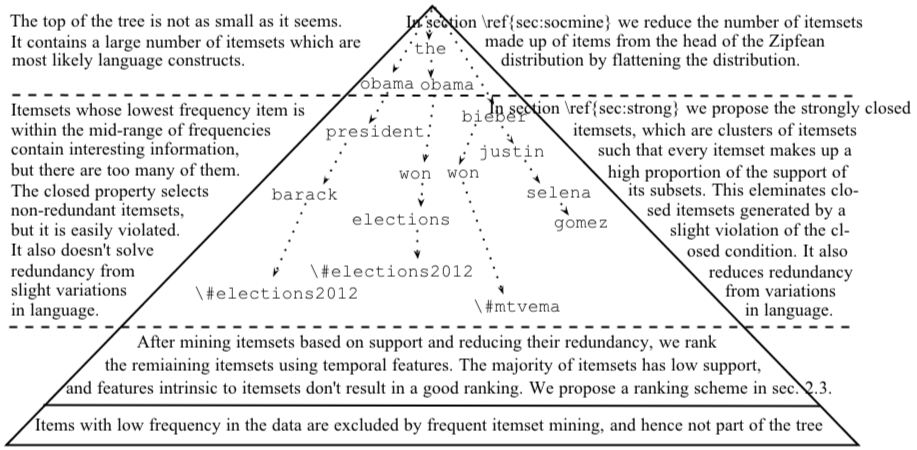
\includegraphics{pyramid-road-map.png}
}
\caption{Most important contributions overlaid on a frequency ordered prefix tree}
\label{fig:outline}
\end{figure}
\end{landscape}


%=====================================




\chapter{Background and Related Work}
\label{sec:related}

\section{Frequent Itemset Mining}
Frequent itemset mining comprises a large body of work that goes back to the
early 1990s~\cite{agrawal1993mining}. 
%A variety of algorithms have been proposed, and they work in totally different ways. 
We categorize frequent itemset mining algorithms into 
algorithms that operate in the item space, 
algorithms that operate in the transaction space, 
and algorithms that operate in the solution space. 
While a comprehensive survey is beyond the scope of this thesis, 
we discuss at least one representative from each category of algorithms.

\subsection{The Apriori Algorithm}
%Frequent itemset mining was proposed 
% was 
%The Apriori algorithm is the first efficient algorithm for frequent itemset mining~\cite{agrawal1994fast}, 
%proposed by Agrawal et al. as part of the solution to the problem of association rules mining. 
%It's goal was finding itemsets that can be broken into a precedent and an antecedent
Agrawal et al.~\cite{agrawal1994fast} proposed the Apriori algorithm 
as part of the first efficient solution to the problem if association rules mining~\cite{agrawal1993mining}.
In the domain of market basked data, 
an association rule is an implication that an item is likely to be purchased
in the same transaction with a certain set of items.
Association rules are mined by finding itemsets that co-occur together frequently, 
then producing a rule with each individual item as a consequent to the purchase of the rest of the itemset.
The Apriori algorithm finds frequent itemsets of increasing lengthes iteratively.
It starts by counting frequencies of individual items (itemsets of length 1). 
Then it iteratively increases the length of itemsets.
At each iteration, it generates candidate itemsets of length K (K-itemsets) 
by merging frequent itemsets of length (K-1) ((K-1)-itemsets) 
that differ in only 1 item, 
usually the last item given a certain total ordering of items.
By using only the frequent  (K-1)-itemsets for generating candidate K-itemsets,
many possible K-itemsets are implicitly pruned, 
based on the anti-monotonicity between itemsets' support and length:
all subsets of a frequent itemset have to be frequent. 
However, each candidate has to be explicitly checked to verify that it does not
have any infrequent subsets.

Apriori and algorithms based on it suffer performance degradation 
and  large increases in memory requirement
when the number of distinct items is high.
These limitations are caused by the candidate generation bottleneck.
A large number of candidates can be generated,
especially in early iterations of the algorithm.
Consider, for example, the generation of candidate 2-itemsets from a database.
This generation requires producing all unordered pairs of 1-itemsets (terms),
after pruning out rare ones with frequency less than the support threshold.
In many domains, including text mining, the number of frequent 1-itemsets is
large enough to prohibit generating a number of candidates in the order of this
number squared.
In text mining, a rather low support threshold has to be used, because the
frequency of terms follow a long-tailed Zipfean distribution.

The Apriori based family of algorithms operates in the item space 
in the sense that an itemset can be expanded by any item regardless
of whether there is any support for the combination. 
%Its efficiency comes from using the current solution to prune out
Operating in the transaction space avoids this blind enumeration
of unsupported candidates, and the subsequent DB scan required 
to count the support of those candidates. 
This involves the creation of a succinct representation of the DB
that is well suited for itemset mining.

\subsection{The FP-Growth Algorithm}
The first algorithm proposed based on the idea of avoiding candidate
generation was FP-Growth~\cite{han2000mining}.
%and traversing a data structure instead
The database is represented as a frequency ordered prefix tree called the FP-tree.
Items with low support are removed, so that 
any node in the FP-tree is necessarily an item with enough support.
An FP-tree imposes the invariant that within each branch the frequency is
non-increasing from the root down to the leaves. 
This increases the chance of finding common prefixes.
%Nodes that are
An FP-tree also contains links between nodes representing the same item.
Those links are used to create the \emph{conditional} FP-tree for an item,
%which is the FP-tree where this item is the root.
which is the FP-tree made only from branches containing this item, 
excluding any items with lower frequency.
The algorithm proceeds by iterating over items in increasing order 
of frequency. 
%For each item, (1) it is output as an itemset,
%and (2) its \emph{conditional} FP-Tree is created and recursively mined. 
Each item is first output as an itemset,
and then its \emph{conditional} FP-Tree is created and recursively mined. 
At each recursive call, the current item is appended to a growing prefix,
which is prepended to all itemsets mined from the conditional FP-tree.
Figure \ref{fig:fpgrowth}, borrowed from Han et. al~\cite{han2004mining}, shows a few steps in the FP-Growth algorithm.
%during the call.

While the navigation of a representation of the database directly
derives itemsets from the transaction space, 
the creation of such representation is a bottleneck itself. 
Building conditional pattern bases and sub-FP-trees becomes very time and space consuming as the recursion goes deep and the number of patterns goes large~\cite{wang2002top}.
%Many alternate representations as well as enhancements to the original FP-Growth
%algorithm were proposed~\cite{cats.....}, however they still operate in the same way.

\begin{figure}%[h]
\centering
\scalebox{0.3}{
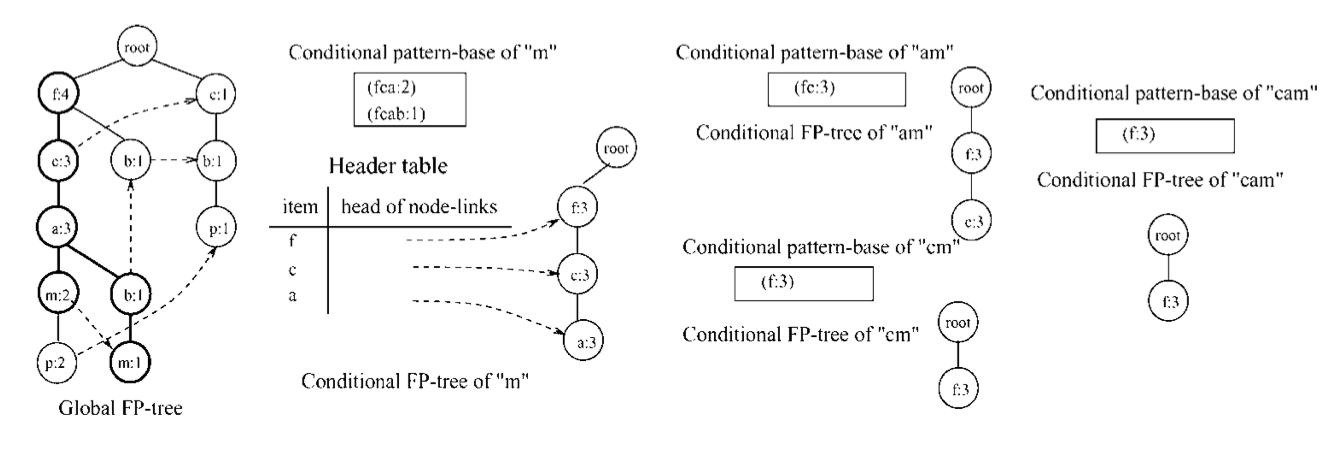
\includegraphics{fp-growth_han-2004.png}
}

\caption{A few steps in the FP-Growth algorithm as depicted by Han et al.~\cite{han2004mining}}
\label{fig:fpgrowth}
\end{figure}

\subsection{Solution Space Algorithms}
\label{sec:sol_space_algs}
The last category of frequent itemset mining algorithms comprises algorithms that operate in the solution space. 
It can be argued that algorithms that traverse a representation of the DB are operating in the solution space rather than the transaction space~--~given that they avoid generating candidates with low support. 
However, in our categorization we focus on the logic behind how itemsets are generated or pruned rather than the data structure used to generate them.
After all, any algorithm must calculate the support of itemsets, and this needs either maintaining a representation of the DB or scanning the transactions. 
Algorithms that operate in the solution space prune itemsets that do not possess certain properties. 
The limited number of itemsets that possess the desired property are sufficient to deduce the rest of the solution (other frequent itemsets and their support).
The reduction in the number of itemsets mined improves the performance of such algorithms, 
even if they rely on candidate generation to enumerate possible itemsets before checking for the desired property.
It is not always necessary to produce the full solution 
since the properties usually filter out only redundant itemsets, 
and in many cases the elect itemsets can be used directly.

%The elect itemsets can be used directly, since the properties usually filter out 
%%to creates a concise representation of the solution 
%%by removing redundancy.
%redundant itemsets only.

The \emph{closure property}~\cite{pasquier1999discovering,pasquier1999efficient,zaki2002charm} prunes an itemset
if it has the same support as its supersets. 
It is easy to see that all itemsets and their support can be derived from the set of \emph{closed} itemsets. 
A formal proof is given by Pasquier et al.~\cite{pasquier1999discovering}.
The smallest itemset of an equivalence class of itemsets having the same support
is called a \emph{generator}~\cite{kryszkiewicz2001concise} or a \emph{free set}~\cite{boulicaut2000approximation}. 
It is also possible to keep only the generator of each equivalence class, 
but in this case some infrequent itemsets has to be kept 
in order to be able to calculate the support of all frequent itemsets~\cite{kryszkiewicz2001concise}. 
A different selection of itemsets can be made according to the Non-Derivable property~\cite{calders2002mining,calders2007non}, 
which is linked to the closed property. %former properties. 

Finding closed itemsets can be done by arranging possible itemsets into a Galois lattice, 
then traversing the lattice using the Galois connection between itemsets and transactions
in which they appear. 
Figure~\ref{fig:lattice} shows an example of a Galois lattice. 
The Galois connection is a pair of operators, one to map an itemset to transactions in which it appears, 
and another to map a set of transactions to the largest itemset that appears in all of them.
Applying the two operators in cascade grows an itemset directly to its closed superset.
More details can be found in Pasquier et al.~\cite{pasquier1999efficient} and Zaki et al.~\cite{zaki2002charm}.

\begin{figure}
\centering
\begin{tabular}{|c|p{1.7cm}|}
\hline
TID&Items\\\hline
1&A B C\\
2&B C E\\ 
3&A B C E\\
4&B E\\
5&A B C E\\
\hline
\multicolumn{2}{c}{The transaction database}\\
\multicolumn{2}{c}{}\\
\end{tabular}
\scalebox{0.5}{
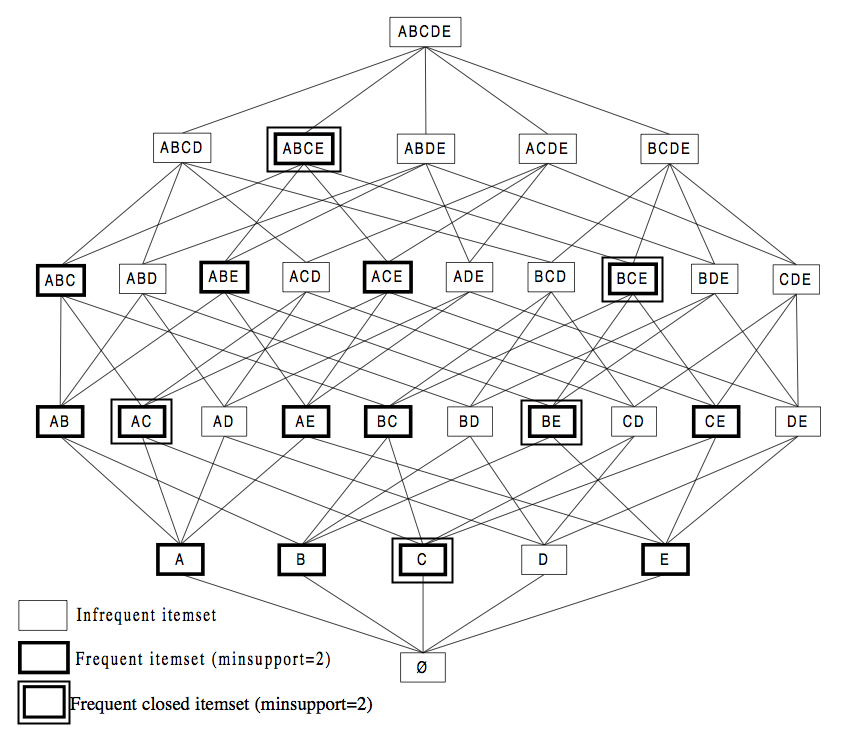
\includegraphics{galois-lattice.png}
}
\caption{Example of a Galois lattice adapted from Pasquier et al.~\cite{pasquier1999efficient}}
\label{fig:lattice}
\end{figure}

Some algorithms take advantage of the closure property to 
reduce the search space more dramatically,
such as CLOSET~\cite{pei2000closet}
and LCM~\cite{uno2004lcm}.
Our work is based on LCM (which stands for Linear-time Closed itemset Mining)~\cite{uno2004lcm}.
As a starting point for our work, we use the implementation of LCM submitted
to the workshop for Frequent Itemset Mining Implementations (FIMI) in
2004~\cite{DBLP:conf/fimi/2004}, which was the workshop's award winner. 
This algorithm is robust against data sparsity, 
and has low memory requirements 
since it does not store intermediate results.
We will explain the closure property and describe LCM in detail in  section \ref{sec:lcm}. 
We proceed by discussing other areas of related work.

%-------------------------------------------------------

\section{Election of Representative or Interesting Itemsets}

The problem of having many itemsets, with redundancy and noise, can be addressed by
picking out  representative itemsets that satisfy a certain condition.
%based on the conciseness or interestingness or the selection.
The representative itemsets are not necessarily sufficient to
deduce the rest of the solution (itemsets and their support information).
In this thesis we propose two conditions for selecting interesting itemsets;
\emph{distinct} itemsets and  \emph{strongly closed} itemsets.
Related approaches to picking out representative itemsets are %: 
choosing a set that will minimize the reconstruction error of the full solution, 
and limiting the number of itemsets to a user specified number.


%Most similar to the \emph{distinct} itemsets we propose in this thesis
%Choosing $\delta$-free~\cite{boulicaut2003free} or 
% $\delta$-covered~\cite{xin2005mining} itemsets are

The $\delta$-free~\cite{boulicaut2003free},  
$\delta$-covered~\cite{xin2005mining}, and 
\emph{master} itemsets~\cite{yan2005summarizing} 
are examples of conditions motivated by providing a compressed representation
of itemsets through sacrificing support information.
The $\delta$-free condition selects an itemsets if its support
is different from the support of all its subsets at least by $\delta$.
This selection of itemsets can be used to approximate the support 
of other frequent itemsets with a guarantee on the error,
but only if some infrequent itemsets are included in the selection.
The $\delta$-free condition implies setting an upper bound on the
strength of association rules that can be derived from selected itemsets.
It is suitable for compressing mining results from dense datasets,
but it is exactly the opposite of \emph{distinct} itemsets we propose in this thesis.


The $\delta$-covered condition is also the opposite of the \emph{distinct}
condition, as it ``relaxes the closure condition to further reduce pattern
set size'' \cite{liu2012finding}. On the other hand, the \emph{distinct}  condition strengthens the closure condition.
The $\delta$-covered condition sets an upper bound on the confidence of the rule that 
an itemset implies a superset; 
if an itemset implies its superset with confidence greater than $\delta$, 
then it is considered to be covered by the superset and can be pruned.
On the other hand, the \emph{distinct} condition
%selects only itemsets that are implied by a subset with high confidence.
sets a lower bound on the confidence of a derived association rule.
Nevertheless, the $\delta$-clusters are similar to the \emph{strongly closed
itemset} clusters proposed in this thesis. 
The efficient version of the clustering algorithm proposed by Xin et al.~\cite{xin2005mining}, RPLocal, 
limits the search space for clustering candidates using a similar reasoning to 
the reasoning used in our algorithm~--~exploiting the sequence in which frequent itemsets are found.
The difference between $\delta$-clusters and \emph{strongly closed itemset} clusters
is that $\delta$-clusters are soft clusters, while \emph{strongly closed itemset} clusters
are hard clusters. 
Also, the distance measure used in $\delta$-clusters is the Jaccard distance,
while the \emph{strongly closed itemset} clusters are based on association rule confidence.

Yan et al.~\cite{yan2005summarizing} proposed a method to choose K \emph{master} itemsets as representatives of the itemsets. 
However, rather than leaving K as a user specified parameter
a method is proposed for choosing K by minimizing the restoration error of support information. %,
%thus it can be considered as a lossy compression approach
A \emph{master} pattern is the union of all itemsets in a cluster, similar to our proposed \emph{strongly closed itemset}. 
While the use of clustering is similarly motivated by the trivial difference between itemsets, the K \emph{master} itemsets  have to cover all itemsets.  
On the other hand,  \emph{strongly closed itemsets}  actually avoid clustering together itemsets representing different topics or different opinions within a topic.
Furthermore, Yan et al. improve performance by approximating the calculation of the distance between itemsets, to avoid accessing the data. 
We can achieve high performance without approximation because our mining results include the postings list of each itemset. 
%we apply clustering to subsets of the data that are very likely to be close to each other.

Another approach to choosing itemsets is according to their interestingness.
The interestingness of itemsets (patterns) has been an area of active research for a long time. 
According to Silberschatz and Tuzhilin~\cite{silberschatz1996makes} interestingness of an itemset
can be \emph{objective} or \emph{subjective}.
Commonly used \emph{objective} measures include (a more extensive coverage is provided by
Geng et al.~\cite{geng2006interestingness}
and Tan et al.~\cite{tan2002selecting}):
\begin{enumerate}
\item \emph{Support}: The number (or fraction) of transactions that contain the itemset
\item \emph{Confidence}: The confidence of a rule derived from the itemset. 
A rule is derived from the itemset by treating one item, $w$, as the consequent of the rule 
while the rest of items, $s \setminus w$, are the antecedent. 
The confidence of the rule is then defined as: 
\begin{equation}conf(s \setminus w \rightarrow s) = \frac{|T_s|}{|T_{s \setminus w}|} \end{equation}
Since different rules with varying confidence can be derived from an itemset, either the minimum (\emph{all-confidence}) or the maximum (\emph{any-confidence}) is used~\cite{omiecinski2003alternative}.
\item \emph{Lift}~\cite{brin1997beyond}: Probability (support) of the itemset over the product of the probabilities of all items in the itemset. This is a measure of dependence and can be linked to Pointwise Mutual Information~\cite{bouma2009normalized}. Such a measure is suitable for Knowledge Discovery or Exploratory Search tasks, where the goal is to extract correlated item sets or significant phrases.
\item \emph{Bond (or Coherence)}~\cite{omiecinski2003alternative}: The support of an itemset over the number of transactions containing \emph{any} of its items.
\end{enumerate}

An important property of a measure, upon which all Apriori based mining algorithm are built, is the downward closure property; 
the value of a downward closed measure cannot increase as the size of the itemset increases.
 All the above measures are downward closed~\cite{bayardo1999mining} with the exception of \emph{lift} which is upward closed 
(cannot decrease with the increase of the size of the itemset), 
and \emph{any-confidence} which is neither upward nor downward closed.
Algorithms that mine itemsets based on the above measures were proposed~\cite{lee2003comine,kim2004ccmine},
but if an application specific measure is to be used then it has to be evaluated in a post mining stage 
or within the Redundancy-Aware Top-K framework~\cite{xin2006extracting}.


The Redundancy-Aware Top-K framework~\cite{xin2006extracting} selects the top K itemsets according to an 
interestingness criterion. % was first %proposed by Xin et al.~\cite{xin2006extracting}. 
The major difference between their approach and all of the previous works is that 
it emphasizes both interestingness and redundancy on the selected top K itemsets, 
and the itemset interestingness is defined in the context of the application; 
summarizing the whole collection of itemsets is not the goal.
Our work fits in the proposed framework: 
we reduce redundancy through filtering and clustering, 
and we propose a ranking that orders itemsets according to some definition of interestingness.
If only the top K itemsets are desired, itemsets ranked at positions higher than K can be omitted.
An explicit number of itemsets needs not be set, however.
This makes our computational model more efficient, 
since we do not need to solve a constrained optimization problem.
In their experiments, Xin et al.~\cite{xin2006extracting} used two application specific interestingness measures:
they used one that is based on TF-IDF for extracting interesting itemsets from a text corpus, 
and another that is tailored for predicting block fetches in storage systems~\cite{li2004c}.
We rank itemsets according to their novelty using a measure based on Information Gain. 
Preliminary experimentation with various other measures of interestingness 
ruled them out as ineffective 
%in the domain of social media. 
for our purposes.

%General as well as application specific interestingness measures were proposedMost of them are

\emph{Subjective} measures of interestingness select itemsets that are actionable or unexpected~\cite{silberschatz1995subjective}.
Selecting unexpected itemsets entails building a probabilistic model to use it for 
estimating itemsets probabilities. 
Jaroszewicz and Simovici~\cite{jaroszewicz2004interestingness} use a Baysian Network as a model,
which is suitable for cases where items are value levels of a limited number of attributes.
A commonly used model is the maximum entropy model~\cite{wang2006summarizing,tatti2008maximum,mampaey2011tell}.
The Maximally informaTiVe itemsets (MTV) algorithm, proposed by Mampaey et al.~\cite{mampaey2011tell},
uses a greedy algorithm to select K itemsets whose probabilities diverge the most 
from the estimate given by a maximum entropy model.
The maximum entropy model is initialized as a uniform distribution.
After selecting each of the K itemsets it is updated 
to fit the selected itemsets actual frequencies
using the Iterative Scaling procedure~\cite{darroch1972generalized}.
If K is set to infinity, the algorithm will generate the best model
according to the Bayesian Information Criterion (BIC). 
Since BIC incorporates a penalty term for the number of parameters
(itemsets included in the model), this selection will  
minimize redundancy while maximizing surprise (divergence from model).
The model can be initialized using itemset frequencies known
from prior knowledge. 
It is also possible to use the Minimum Description Length (MDL)
as a criterion for selecting itemsets.
We compare our selection of itemsets to ones obtained from MTV using 
the implementation provided by the authors\footnote{http://www.adrem.ua.ac.be/implementations}.
However, the value of K has to be kept low (at most 50) for the algorithm to finish without an error, 
even though it is running without a limit on its resource usage on a machine with 256 GB of RAM.
In our work we focus on efficiency, allowing the summary to include larger numbers
of itemsets than the values of K for which MTV is efficient (at most 10). 
This is crucial for scalability to the volumes of data typical in social media streams.

Another approach to picking out itemsets is choosing ones that 
can be used to compress the data. The KRIMP algorithm~\cite{vreeken2011krimp} is 
a good example of methods that follow this approach. Our goal is different because
we aim to filter out itemsets pertaining to personal updates, which make up a large
portion of social media data. 

\section{Frequent Itemsets in Search and Summarization}

Different ways to use Frequent Itemset Mining in search %the field of Information Retrieval 
has been proposed. 
Possas et al.~\cite{possas2002set}  proposed using closed itemsets
in place of terms, using them in exactly the same way as terms are used.
In the tokenization process, they use CHARM~\cite{zaki2002charm} to mine closed itemsets from 
frequent tokens in the document.
They then add the document to the postings lists of each closed itemset
present in the document. 
Queries are tokenized similarly and results are ranked using TF-IDF.
This simple approach achieves increased precision on various test collections, 
possibly because frequent itemsets take into account collocation information.
The approach is so simplistic, however. 
The overlap in closed itemsets was not taken into account while tokenizing documents and queries into itemsets.
Also, the mining algorithm was not modified to accommodate the high number of terms %, 
and the greater length of documents compared to the length of transactions typical to market basket data.
Finally, the number of itemsets is higher than the number of terms so the index size will increase.

Wu et al.~\cite{wu2004automatic,wu2006deploying}
propose the use of sequential closed patterns instead of terms, 
in what they call \emph{pattern based approach} to information retrieval.
They consider patterns as surrogates to phrases that have
better statistical properties than phrases, 
thus achieving a break through in the performance 
of \emph{phrase based approaches}.
``Although phrases contain less ambiguous and narrower meanings than individual words, the likely
reasons for the discouraging performance~\cite{lewis1992evaluation} from the use of phrases are: (1) phrases have inferior statistical properties to words, (2) they have low frequency of occurrence, and (3) there are a large number of redundant and noisy phrases among them.''~\cite{wu2006deploying}
They address the problem of overlap in closed patterns,
and they developed an algorithm specifically tailored for mining closed sequential patterns from text.
Documents are broken into paragraphs which are the unit of mining and retrieval.
This alleviates the problem of having documents that are much longer than traditional market basket transactions.
Albathan et al.~\cite{albathan2012using} extend the work of Wu et al. by 
proposing a method for further reducing the number of closed patterns.
Lau et al.~\cite{laumicroblog} used related methods for term weighting 
in pseudo-relevance feedback for Twitter search,
and achieved substantial improvements over a baseline.
Our work can provide such methods by a short ranked list of itemsets. 


Our work complements the work done by Yang et al.~\cite{yang2012framework} for 
using frequent itemsets as a temporal summary. 
They have proposed a framework for storing mining results of 
temporally consecutive intervals (batches of data) using a pyramidal time window. 
Their framework allows for fast execution of temporal queries, and for tracking the evolution of topics. 
However, the itemsets stored for each interval is not selected for providing the best summary.
Itemsets are selected according to their utility in a
lossy compression algorithm.
The algorithm is based on representing transactions as itemsets that cover them, 
possibly introducing items that are not originally in the transaction or omitting items from the transaction.
%and it might introduce false positives and negatives. 
%The algorithm could meet the desired  constraints on memory consumption (set at 20MB) and on processing data as a stream, but there was no justification why such tight constraints should be set. On the other hand, 
%The quality of the summary seems to be affected by the choice of utility function, but the only assessment made about this was showing that 
The actual transactions can be reconstructed with an accuracy that is expected to be high 
if the transaction contains ``both recent and frequent keywords''. 
The temporal summary is created from the reconstructed transactions in a separate step.
First, the pyramidal time window is queried using keywords and a specific time intervals 
(for example, ``world cup'' on the day before a certain matche).
Then, non-negative matrix factorization is used to extract topics from the returned transactions.
The pyramidal time window structure can be used to store itemsets
selected by our methods, 
thus directly providing a temporal summary
without the need for the matrix factorization step.
%the data is preprocessed by stemming and stop words removal, 
%which should require a language identification component upstream but it is not discussed.
Our methods exploit the nature of social media to choose topically relevant itemsets without the need for a query. 
Social media has been shown to be a good source of real-time information, as we will discuss in the next section.

\section{Social Media as a Source of Information}

The problem of finding information in social media posts 
%is an active area of research bec
is motivated by the uniqueness and variety of information that can be found
in these media. 
Some stories are reported mainly on social media 
because 
of censorship on journalism, 
such as the 2009~-~10 Iranian election protests 
(nicknamed ``Iran's Twitter Revolution''
\footnote{http://www.theatlantic.com/technology/archive/2010/06/evaluating-irans-twitter-revolution/58337/}).
Other stories are reported mainly on social media
because of the 
content creator happens to be at the right place
at the right time. 
This could be by chance like in the case of
the emergency landing of a US Airways plane 
on the Hudson river in New York
\footnote{http://www.telegraph.co.uk/technology/twitter/4269765/New-York-plane-crash-Twitter-breaks-the-news-again.html}.
This could also be an intentional act
of citizen journalism. 
Citizen journalists are ``the people formerly known as the audience,'' who ``were on the receiving end of a media system that ran one way, in a broadcasting pattern, with high entry fees and a few firms competing to speak very loudly while the rest of the population listened in isolation from one another~--~ and who today are not in a situation like that at all. "
%... The people formerly known as the audience are simply the public made realer, less fictional, more able, less predictable.''
\footnote{http://archive.pressthink.org/2006/06/27/ppl\_frmr.html\#more}.

In a study of the use of Twitter as a news medium during the 2011 Tunisia and Egypt revolutions, 
Lotan et al.~\cite{lotan2011revolutions}  categorized 963 accounts that made influential posts according to the \emph{type of actor}. 
A post is considered influential if it is among the top 10\% of posts in terms of the number of near duplicates made out of it; 
posts that had at least 16 near duplicates in the Tunisia data, or at least 19 near duplicates in the Egypt data.
The types of actors included Mainstream Media organizations and Mainstream New Media organizations, 
which are news and media organizations with and without offline presence, respectively.
It also included Journalists, who are individuals employed by media organizations or who 	regularly work as freelancers for them.

In both datasets, media organizations make up about 11\% only of these accounts (approximately 7\% for ones with offline presence and 4\% for ones that exist solely online). 
Journalists make up another 15\%, so the total of mainstream media affiliated accounts is approximately 26\%.
On the other hand, more than half of the accounts from which influential tweets originated belong to individuals not affiliated to the government or mainstream media (55\% for Tunisia and 56\% for Egypt). 
Out of those individual, almost half are ordinary people who don't self identify and cannot be identified by assessors as bloggers or activists. 

The rate at which an account makes posts is approximately 16 per hour for mainstream media affiliated accounts, and approximately 10 for individuals accounts (thus a mainstream media account makes 60\% more posts). 
Also the probability that a post will be echoed is 0.88 for mainstream media accounts, 0.55 for journalists, 0.4 for bloggers and activists, and 0.31 for individuals 
(this is the probability that any follower will echo the post, the average number of followers of all types of actors is much higher than that of ordinary people).
However, collectively the fraction of highly echoed threads originating from ordinary people is on a par with 
the fraction of threads originating from a journalist. 
Threads originating from ordinary people, bloggers and activists together make up more than half of highly echoed threads, followed by threads originating from journalists (around 20\%), then threads originating mainstream media (around 10\%, divided equally between media with and without offline presence). 

All this emphasizes the influence citizen journalists and ordinary people now have on 
the information creation and dissemination process.
User created content is rich with unique content tackling a variety of topics from different points of view.
However, it is dominated by non-informative chatter and personal updates. 
In a study comparing the use of Twitter's search feature to Web search, 
Teevan et al.~\cite{teevan2011twittersearch} found that
Twitter is mostly used for getting timely information:
updates about events, 
news about topics of interest (such as technology news),
and realtime local updates (such as traffic jams).
It was noted that Twitter search could be the main
way of accessing Twitter, since posts from the followed network 
could to be outside of the user's topical interests. 
This is supported by findings from an earlier study by
Naaman et al.~\cite{naaman2010really} in which
3379 tweets from 350 accounts belonging to individuals
were studied. 
The tweets were hand coded into different categories, 
then the activity of users in terms of
what type of tweets they make was analyzed.
It was found that 40\% of the studied tweets 
are personal updates (about ``Me now''),
and that users can be clustered into
a big cluster of ``Meformers'' 
(80\% of the users, half of their posts are personal updates)
and a small cluster of informers 
(20\% of the users, half of their posts are for sharing information).
The study also found that most people engage
in some form of Meformer activity; 
on average, users had 41\% of their messages
in the ``Me now'' category.
Therefore filtering out posts by Meformers, 
or giving higher weights to posts by Informers 
will not be enough for finding informative posts
made by ordinary people.

To tap into social media as a source of information, 
social media users collaboratively select good content.
On Twitter, users can \emph{retweet} an interesting post, 
which means forwarding it to their followers.
The dynamics of retweeting was studied by Boyd et al~\cite{boyd2010tweet}.
One of the findings was that posts being retweeted 
are frequently modified to accommodate additional 
text, or at least the notation meant to indicate 
that the message is a retweet. 
This is because Twitter limits tweets to 140 characters.
The selection of what to keep from the post is actually 
a form of collaborative filtering itself, 
because the most interesting parts has 
to be retained. 
The parts that are selected by many people
is likely to be a good summary of what is interesting.
The words in this part would make up a frequent itemset.
Other methods for finding emerging topics in social media
are discussed in the next section.
%also make use of the unusual frequencies of such collocation. 

%\section{Exploratory Search and Topic Summarization for Social Media}
\section{Topic Detection and Tracking for Social Media}

The problem of Topic Detection and Tracking (TDT) was introduced by Allan et al. in 1998~\cite{allan1998topic}.
%and the community defined five tasks that a TDT system should be able to perform: 
%\emph{Topic Tracking, Link Detection, Topic Detection, First Story Detection and Story Segmentation}.
%Out of those tasks Topic Detection is the most releted to our work, but the rest are also related. 
Topic Detection is the discovery of previously unknown topics, 
where a topic was first defined as an ``event'' then 
its definition was broadened to include the triggering event 
as well as 	other events and activities directly related to it.
%Topic Tracking is
Our work can be categorized as a method for topic detection from social media,
or more specifically ``event'' detection since we make no effort to group events into topics.
%Even though TDT was introduced long ago, it has been an area of active research ever since.
Ever since it was introduced, TDT has been an area of active research.
Besides the fact that there is always room for improvement, 
TDT was originally targeting the domain of newswire data, 
and the solutions developed for this domain are not directly applicable to 
data from other domains. 

In the domain of social media, Petrovi\'{c} et al.~\cite{petrovic2010streaming}
used an adaptation for Locality Sensitive Hashing (LSH)~\cite{indyk1998approximate} to
perform first story detection at scale. 
The computation framework is the same as the one
used in traditional systems~\cite{yang1998study,allan2000detections}.
For each tweet find the nearest neighbour in the vector space of terms. 
If the distance is less than a threshold then add the document to the topic represented by the cluster containing the nearest neighbour.
Otherwise, create a new cluster representing a new topic. 
The current document is the first story of the topic.
The adaptation to LSH that they propose reduces 
the number of times a document is considered far
from all its neighbours while it actually is not.
They do that by comparing the document to 
%a fixed number of documents that are posted
%within the 
the last 1000 tweets, and update the minimum distance if necessary.
Using LSH, with the adaptation, didn't affect the quality of results much 
as compared to the UMass FSD system~\cite{allan2000detections}
on a traditional TDT task (TDT-5).
On the other hand, the run time was decreased from 28 hours to 2 hours.
The UMass system could not finish processing a dataset 
of a 160 million tweets
collected over a period of 6 months from Twitter,
while their proposed system can process each
tweet in bounded space and time.
One problem remains, however.
The precision of determining if a tweet cluster
is actually pertaining to an event or just normal chatter
or spam is low. 
Actually their system can detect spam clusters
with high precision ($average\,precision=0.963$), but not events ($average\,precision=0.34$).
The problem of identifying event clusters was further studied by Beker et al.~\cite{becker2011beyond},
where they used a Support Vector Machine (SVM) classifier and achieved a higher precision.
However, their test set was limited to 5 hours of Twitter data and the precision decreases as 
the number of clusters increases because the classifier is trained on the positive case.
%of about 0.65 correctly classified event clusters out of 20 clusters.

Another method of event detection follows the framework of bursty keywords detection proposed by Kleinberg~\cite{kleinberg2003bursty}. %, for topic detection in e-mail streams. 
In this framework, a set of keywords are tracked~--~possibly all tokens in the dataset.
A state machine is used to indicate the stat of each keyword, 
where consequitive states correspond to higher levels of \emph{burst} intensity. 
Each transition between states is associated with a cost, 
and a keyword moves between the states to minimize the overall cost of its transitions.
A simplified version of this framework is use by Parikh and Karlapalem~\cite{parikh2013events},
where there are two states for each token. 
A token is moved to the state of being bursty
if the increase in its frequency exceeds a threshold,
and it stays in this state for a fixed time interval. 
The bursty tokens are then clustered into events.
%is higher than the increase between all other intervals.
%the difference in the frequency of each token is tracked in of fixed span and keywords are considered bursty
Another method that tracks the frequency of all tokens is EDCoW~\cite{weng2011event}, 
where the wavelet transformation is used to convert counts of occurrences from the time domain to the frequency domain
then auto-correlation is used to detect burstiness.
However, the use wavelet transformation is not justified
specially for the enormous number of tokens in case of social media.
Other methods based on burst detection track a small set of keywords. 
Lehmann et al.~\cite{lehmann2012dynamical} track hashtags and study 
their usage pattern.
Chakrabarti and Punera~\cite{chakrabarti2011event} track 
tokens appearing in tweets tagged by an American Football team name,
and use them to create a summary of the game.

Our work can be seen in the light of Meme-tracking~\cite{leskovec2009meme},
where a particularly interesting quotation (meme) is tracked across news and blog posts.
The quotation being tracked is not quoted verbatim in all posts, 
but rather parts of it are selected and it could be slightly paraphrased.
This is similar to modifications made during retweeting an interesting tweet.
Leskovec et al.~\cite{leskovec2009meme} tracked quotations made by
American politicians during the 2008 U.S. presidential elections.
Phrases made up of 4 words or more are tracked if they got repeated 10 times or more,
where at most 25\% of the repetitions could be on the same domain name.
A directed acyclic graph is constructed where phrases are vertices 
and edges are weighted according to the edit distance between phrases, 
as well as the number of occurrences of the longer phrase.
The graph is then divided into clusters where each cluster contains
one \emph{root} that has no outgoing edges. 
Each vertex is assigned to the cluster 
with which it has the highest number of edges.
Clusters are then ranked according to the number of news and blog posts 
containing any phrase from the cluster.
Leskovec et al. then use the clusters and their associated news and blog posts
to perform an analysis of the temporal variation of the volume of posts about
each meme.
They propose a model that fits the data well, 
and study the difference between blog posts and news.
In our work, we are also using the volume of posts 
containing phrases and their variations (itemsets).
We also do clustering but in a different way, 
and we work in a totally different scale of time.

O'Connor et al.~\cite{o2010tweetmotif} also start from phrases
to summarize tweets about a user specified query.
They select \emph{significant} phrases which
are statistically unlikely, then cluster them. 
Frequent itemsets are a better starting point than phrases,
since there are much more phrases than frequent itemsets.

Event detection in Twitter can also be done using 
Natural Language Processing
to identify \emph{event} parts of speech~\cite{ritter2012open},
or to identify action phrases~\cite{popescu2011extracting}.
Of course, it is also possible to apply topic modelling 
by Latent Dirichlet Allocation (LDA)~\cite{hong2010empirical}
or an online varient~\cite{hoffman2010online,yao2009efficient}.
Our method tackles the problem in a totally different way.

% ===================================
% ===================================
% C H A P T E R     3	
% ===================================
% ===================================
\chapter{Mining Social Media Text}
\label{sec:socmine}


\section{The Linear-Time Closed Itemset Mining \\Algorithm}
\label{sec:lcm}
In section~\ref{sec:sol_space_algs} we have discussed frequent itemset mining algorithms that
overcome the bottleneck of \emph{candidate generation} by 
limiting the solution to itemsets with a certain property, 
reducing the size of the solution and 
possibly providing a way to quickly navigate the solution space. 
In this thesis, we expand on the Linear-time Closed itemset Mining (LCM) algorithm \cite{uno2004lcm}, 
%an algorithm based on a
%property of a class of itemsets called
which mines only 
\emph{closed itemsets}~\cite{pasquier1999discovering}.
The  LCM algorithm is distinctively fast because it also 
takes hints from the transaction space 
during candidate generation.
%Generating candidates according to information from the transaction space
This also makes it resilient against data sparsity,
since it will not consider a candidate that never appears in the data.
The ability to efficiently mine sparse data makes LCM particularly
suitable for mining social media text.
In this section we explain in detail how LCM works.

Since LCM makes use of the properties of closed itemsets, 
we begin our presentation by discussing these properties.
Informally, a closed itemset contains any item that is present in all the transactions
containing this itemset.
A formal definition of closed itemsets is given in equation \ref{eq:Closed}: 

\begin{equation}\label{eq:Closed}\mathcal{C} = \{s_c:\, s_c \subset W \, and \,\nexists \, s_d \, where \, s_c  \subset s_d \, and \, |T_{s_c}| = |T_{s_d}|\}\end{equation}

The properties of closed itemsets are as follows:
\begin{enumerate}
\item Adding an item to a closed itemset reduces its support. 
\item A subset of a closed itemset is not necessarily closed, but one or more closed subset must exist for any itemset (formally this could be the empty set, given that any item that appears in all transactions is removed in a preprocessing step). 
\item If a closed K-itemset can be extended any further then one of its supersets will be closed, however not necessarily a (K+1) superset. Itemsets that cannot be extended any further are called \emph{maximal itemsets}, which form a subclass of closed itemsets.
\end{enumerate}

Besides being much smaller than the solution space of frequent itemsets,
the solution space of closed itemsets can be navigated efficiently.
By using an arbitrary total ordering of items, any closed itemset can be
considered an extension of exactly one of its subsets.
Thus, only this subset is extended during candidate generation.
All other subsets do not need to be extended by items that would lead to
the longer closed itemset.
This property is called \emph{prefix preserving closure extension
(PPC-Extension)} and it was proposed and formally proved by
Uno et al.~\cite{uno2004lcm}.


\emph{PPC-Extension} is achieved by following three rules, which we state
after a few definitions to facilitate their statement.
First, an item is \emph{larger/smaller} than another item if it comes
later/earlier in the total ordering.
This terminology comes from the fact that LCM is most efficient if the items
are ordered in ascending order of their frequency.
Second, the \emph{suffix} of an itemset is one or more items 
%whose removal results in
%does not result in
which have to be removed to get
an itemset with greater support.
Notice that they are necessarily 
%at the end of the itemset,
the last items added to the itemsets,
regardless of the total ordering.
Finally, we call the first item added to the suffix of the itemset its
\emph{suffix head}.
With this terminology, the rules for \emph{PPC-Extentsion} are:
\begin{enumerate}
\item An itemset must be extended by all items that occur in $T_{itemset}$, 
except items which are \emph{smaller} than its \emph{suffix head};
extending by \emph{smaller} items will lead to closed itemsets already generated in an earlier step. 
%An itemset can be extended only by items \emph{larger} than its \emph{suffix head}; 
%extending by \emph{smaller} items will lead to closed itemsets already generated. 
%Each itemset must be extended by all the qualified items that occur in $T_{itemset}$.
Extension items are added to the itemset in the order given by the total ordering,
%and the maximal itemset 
recursively applying PPC-Extension to the extended itemset before adding the next extension item.
\item After forming an itemset $s$, we add to its \emph{suffix} all items that appear in all transaction containing $s$ ~--~ 
that is, items whose frequency within  $T_s$ is equal to $|T_s|$.
%\item If any item in the \emph{suffix} is \emph{smaller} than the suffix head, prune this solution branch. All closed itemsets within this branch have already been generated. Otherwise emit solution.
\item If all items in the \emph{suffix} are \emph{larger} than the \emph{suffix head} then add the itemset to the solution. Otherwise, prune this solution branch; all closed itemsets within this branch have already been generated, when processing the smallest suffix member.
\end{enumerate}
 
Table \ref{table:PPCExample} is an example of how \emph{PPC-Extentsion} is
used to generate closed itemsets starting from the
\emph{1}-itemset \{`barack'\}.
The upper table enumerates $T_{\{barack\}}$.
The lower table shows steps of itemsets generation.
The current itemset along with its frequency is in column 2.
Itemsets marked by an (*) are the closed itemsets that are part of the solution.
The suffix of the itemset is shown in \emph{italic} when it is important to make it distinctive.
All possible extension items and their frequencies are in column 3. 
Extension items that are \emph{smaller} than the \emph{suffix head} 
%are excluded by striked through.
are shown with a line striked through them.
For each itemset, the extension items are kept 
so that it is known which extension item 
is next in turn to be added.
An item is bolded when it is added because its turn has come. %The item being added
%Column 4 is a comment explaining the step.
After adding each item, a pass is done on $T_{itemset}$ to 
enumerate and count possible extension items.
To enforce a support threshold infrequent extension items would be removed
after counting, %at this time,
but in this example there is no such threshold.
Finally, column 4 is a comment explaining each step.

%Notice
Table \ref{table:PPCExample} shows that the number of steps is linear in the number of closed itemsets,
and the only additional storage required, besides storage for the documents,
is that required for possible extension items.
Of course, this is a simplified example, but it shows in essence how LCM
achieves its low run time and memory requirements.
We refer the interested reader to Uno et al.\cite{uno2004lcm} for a
theoretical proof that the algorithm runs in linear time in the number of
closed itemsets,
and that this number is quadratic in the number of transactions.
Performance on a real data set is shown in section \ref{sec:socmine}.
We proceed by describing how to implement this algorithm using an inverted
index.

\begin{landscape}
\begin{table}
\centering
\begin{tabular}{|c|p{5cm}||c|p{5cm}|} \hline
Doc. Id & Document & Doc. Id & Document\\\hline
a& barack \& mitt & b & brack obama \& mitt romney  \\\hline
c& brack obama \& romney & d & brack obama  \\\hline
\end{tabular}
\begin{tabular}{c}
Documents (two per row)\\\\
\end{tabular}
\begin{tabular}{|c|p{6.5cm}|p{6.2cm}|p{7.6cm}|} \hline
Step&Current Itemset&Possible Extension Items&Comments\\ \hline
1& \{\emph{barack}\} (4) & mitt (2), obama (3), romney (2) & Items in $T_{\{`barack'\}}$ are counted. No items should be added to the suffix.  \\ \hline %with `barack'
%appears in all transactions.%
%This is not shown as a step in the rest of the example.
2& \{barack\} (4)* & mitt (2), obama (3), romney (2) & Rule 3: suffix is ordered, add itemset to solution. This is not shown as a separate step in the rest of the example.\\ \hline
3& \{barack\} (4) & \textbf{mitt} (2), obama (3), romney (2) & Items are ordered lexicographically. Adding `mitt' to itemset.\\ \hline
4& \{barack, \emph{mitt}\} (2)* & \textbf{obama} (1), romney (1) & Extension items reenumerated \& counted.\\ \hline
5 & \{barack, mitt, \emph{obama}\} (1) & romney (1)                       & Rule 2: `romney' appears in all $T_{itemset}.$\\\hline
6 & \{barack, mitt, \emph{obama, romney}\}(1)* & & Rule 2: `obama'  is the \emph{suffex head}. \\\hline
7 & \{barack\} (4) & mitt (2), \textbf{obama} (3), romney (2) & Nothing more to add, back to \{`barack'\}. \\\hline
8 & \{barack, \emph{obama}\} (3)* & \sout{mitt} (1), \textbf{romney} (2) & Rule 1: skipping `mitt', adding `romney' \\\hline
9 & \{barack, obama, \emph{romney}\} (2)* & \sout{mitt} (1) & Rule 1: Nothing more to add. \\\hline
10 & \{barack\} (4) & mitt (2), obama (3), \textbf{romney} (2) & Back to \{`barack'\}, adding `romney'. \\\hline
11 & \{barack, \emph{romney}\} (2) &  \sout{mitt} (1), obama (2) & Rule 2: add obama to suffix after `romney'. \\\hline
12 & \{barack, \emph{romney, obama}\} (2) &  \sout{mitt} (1)  & Rule 3: suffix is not ordered, prune. \\\hline
13 & \{barack\} (4) & mitt (2), obama (3), romney (2) & Back to \{`barack'\}, all possible extension items were added. Done. \\\hline
\end{tabular}
\begin{tabular}{c}
Closed itemsets containing `barack'
\end{tabular}
\caption{Generation of closed itemsets by Prefix Preserving Closure Extension}
\label{table:PPCExample}
\end{table}
\end{landscape}

\subsection{Implementation Details}
We show in algorithm~\ref{algo:lcmix} how to implement LCM and PPO-Extension
using an inverted index.
The algorithm assumes the presence of a search infrastructure,
with the ability of performing boolean queries efficiently.
Besides the high likelihood that such an infrastructure already exists,
it is also a very good representation of textual data.
%It provides a more succinct rep
%We experimented with other representation that are designed to provide 
Other representations that are designed for databases in general
might not be well suited for textual data. %,from the nature of .
For example, the memory requirements of the FP-tree suffers from the sparsity
of data, since the data structure is succinct only if it can find common
prefixes within the constraints of its invariant. 
The possibility of using an inverted index in the implementation 
of LCM is yet another reason why it is very well suited 
for textual data.
%for frequent itemset mining from 

The algorithm takes as input an epoch of data and a support threshold as a
ratio $\alpha$.
%The ratio is sp
It outputs the closed itemsets with support above the threshold.
Along with each itemset in the solution, it also outputs the transactions
in which it occurs~--~which is represented as $\langle items,
T_{itemset} \rangle$.
The symbol $\succ$ denotes that the lefthand side  succeeds the righthand
side in the total ordering.
In the implementation shown, it is not necessary that the inverted index's tokens  list (X.tokens)
follow the total ordering; all itemsets of length 1 will be considered anyway. 
Each 1-itemset is then expanded according to the PPO-Extension rules.
Lines 11-18 are the enumeration and occurrence counting of possible extension items, 
except line 15 which forms the closed itemset according to PPO-Extension rule 2.
Lines 19-20 prunes a solution branch according to the rule 3, 
and line 21 adds the itemset to the solution according to the rule's complement.
Lines 22-27 extends the itemset according to rule 1, 
where line 23 (along with line 5) enforces the support threshold.


The algorithm lends itself to distributed implementations.
For example, a map/reduce implementation is straightforward since the only
operations are counting (line 15) and projection (line 24).
However, the fast execution time and the low memory requirements of the
algorithm makes it possible that a distributed implementation will
cause unnecessary overhead for all but the largest data sets.
We experimented with Hadoop\footnote{http://hadoop.apache.org}
%, an open source map/reduce framework, 
and the overhead was in the order of minutes.
Besides, many problems start to arise 
when the programming model is complicated,
and Hadoop was particularly problematic.
%Intermediate results has to be read and written from disk multiple times,
%and might even be copied over the network. 
%Using data management components from the Hadoop ecosystem
%didn't help in achieving a speed up. 


\begin{algorithm}
\SetAlgoLined
\LinesNumbered
\SetKwProg{Fn}{Function}{ is}{end}
\KwIn{$support$: Support threshold} %Dynamic

\KwData{E: Epoch of data}
\KwResult{C: Closed itemsets occurring  in at least $\alpha * |E|$ records}
C $\gets \{\langle \emptyset, E\rangle\}$ \tcp*{$\emptyset$ is a closed itemset. This is skipped in practice}
X $\gets$ Inverted index of E\;
\ForEach{$w \in X.tokens$}{
	$T_{\{w\}} \gets$ X.postingsList[$w$]\;
	\uIf(\tcp*[f]{Support threshold for 1-itemsets}){$|T_{\{w\}}| \geq support$}{ %\alpha * |E|$}{ %\frac{|E|}{E.span}
		LCM($\{w\}, w, T_{\{w\}}$) \;
	}
}
\Return{C}\;

\Fn{LCM(s: Current itemset,   $w_{sh}$: Suffix head, \\ \hspace*{1.2in}$T_s$: Transactions (tweets) containing s)}{
	frequency[$1 \ldots w_n$] $\gets$ 0\;
	suffix $\gets \{ w_{sh}\}$\;
	\ForEach{$t \in T_s$}{
		\ForEach{$w \in t$}{ 
			frequency[$w$]++\;
			\lIf{frequency[$w$] $ = |T_s|$}{
				suffix.add($w$)%	\tcp*{ PPO-Extension Rule 2}
			}  
		}
	}
	\uIf{$\exists v \in suffix: w_{sh} \succ v$ }{
		\Return \tcp*{Prune according to PPO-Extension Rule 3}
	} 
	C.add($\langle s \cup {suffix}, T_s\rangle$)\;
	\ForEach{$v \succ w_{sh}$ and $v \notin $ suffix}{
		\If{frequency[$v$] $\geq support$}{%\alpha * |E|$}{%\frac{|E|}{E.span}
			$T \gets T_s \cap v$	\tcp*{Results of query $s$ AND $v$}
			LCM($s \cup suffix \cup \{v\}, v, T$) 
		}
	}
}

\caption{The LCM frequent itemset mining algorithm}
\label{algo:lcmix}
\end{algorithm}

%-----------------------------

%\section{Dataset and Data Preprocessing}
\section{Using LCM for Mining Social Media Text}
\subsection{Dataset}
Throughout this paper we use data collected from the Twitter public
stream\footnote{https://dev.twitter.com/docs/streaming-apis/streams/public}
since October 1st, 2012. 
We use only tweets written in the Latin script to facilitate tokenization
using white space and other word boundaries.
We collect only the tweet text to avoid reliance on any features specific to a
certain social medium,
and to make the algorithms applicable to other media where text is short such
as Facebook or Google+ status updates.
%The only preprocessing we performed was to
We remove duplicate original tweets
(not retweets) using a Bloom filter~\cite{metwally2005duplicate}.
This filtering removes spam tweets sent by botnets, averaging at 2.86\% of the stream. 
%3352.61069856614 / 116920.214769629
There were two disruptions during data gathering. 
One in late October because of Hurricane Sandy
which made the Twitter service unaccessible.
The other was in late December because of 
technical problems 
%running out of disk space
on the server gathering the data.
%It took a couple of days for the author to notice
%because he was back home on vacation. 



% select count(*), avg(count), stddev(count) from numtweets_date;
% count |         avg          |     stddev      
%-------+----------------------+-----------------
 %  112 | 2705931.830357142857 | 583705.63189013
%(1 row)
%march=# select count(*), avg(count), stddev(count) from numtweets_date where count > 100000;
% count |         avg          |     stddev      
%-------+----------------------+-----------------
%   109 | 2779091.816513761468 | 385334.92621946
%(1 row)


%march=# select count(*), avg(count), stddev(count) from numtweets_hourly;
 %count |         avg         |     stddev     
%-------+---------------------+----------------
% 2546 | 119035.492930086410 | 24774.95441253
%(1 row)
%march=# select count(*), avg(count), stddev(count) from numtweets_hourly where count > 100000;
% count |         avg         |     stddev     
%-------+---------------------+----------------
%  1948 | 130575.470739219713 | 13980.26111766
%(1 row)
%march=# select count(*), avg(count), stddev(count) from numtweets_hourly where count > 50000;
% count |         avg         |     stddev     
%-------+---------------------+----------------
%  2541 | 119210.870129870130 | 24465.65658672
%(1 row)
%march=# select count(*), avg(count), stddev(count) from numtweets_hourly where count > 25000;
% count |         avg         |     stddev     
%-------+---------------------+----------------
%  2544 | 119123.931996855346 | 24582.24599789
%(1 row)


%From perfmon
%Hourly Volume     | 37049 | 113569.051931226 | 23522.1711336507 | 184661 |   1
%Daily Volume     |   876 |      2532001.33561644 | 425519.560561978 | 3116548 |    1


The average number of tweets per hour  (\emph{volume velocity}) in the data is 119,035.49 tweets 
(n = 2,546 hours, standard error = 491), 
and the average number of tweets per day is 2,705,931.83 tweets 
(n = 112 days, standard error = 55,155). 
These are simple moving averages calculated by summing the number of tweets in 
non-overlapping epochs and dividing by the number of epochs.
%However, the number of tweets 
A more accurate estimate of the average number
of tweets at different hours of the day 
can be acquired using a timeseries model
of the activity on the social network.
% number of tweets %volume velocity 
% at each hour can be calculated using a state space model

\subsection{Timeseries model of the dataset}
Arrivals entering a system are commonly modelled as
a Poisson stochastic process.
A Poisson process can be 
characterized by a random variable $N(t)$ %series of 
representing the aggregate number of arrivals 
that has happened up to time $t$.
This random variable has a Poisson probability mass function
with a rate $\lambda$
(as well as two other necessary properties: independent and stationary increment).
When the rate is high enough (more than 1000), 
the Normal distribution can be used as an approximation
to the Poisson distribution. 
Since social media has arrival rates larger than 1000
posts per minute 
(the time unit is arbitrary but must be long enough to have more then 1000 arrivals),
it is therefore possible to assume a normal distribution
and use a state space model 
to describe the activity on the social network.

Values in time series data is known to be correlated,
and specialized models are developed to deal with such explicit correlation.
The explicit correlation is usually uninteresting, 
since it is known and expected.
For example, the data can be known to have a trend such as a chronic increase in the volume velocity. % of Twitter.
Also, a cyclic increases and decreases in the volume velocity according to the time of day can be expected~-~this is called the seasonal effect in time series analysis.
State space methods provide an explicit structural framework for the decomposition of time series~\cite{commandeur2007introduction}.
%in order to diagnose all the dynamics in the time series data simultaneously 
Unlike the more popular Box~-~Jenkins ARIMA models, 
trend and seasonal effects are not treated as nuisance parameters, 
and it is not necessary to remove the trend and seasonal effects 
from the series before the analysis can begin.
Instead, a state space model has an equation 
to capture each type of effect that is suspected
to contribute to the values of the observed variable.
Different models can be used to describe the same
observed variable, and the best model is
selected using the Akaike information criterion 
which penalizes extra parameters.

After experimentation with different models,
we found that the model that best describes the 
volume velocity of Twitter is the following: %Gaussian Random Walk
\begin{enumerate}
\item A deterministic seasonal cycle that is 1 day long, which captures the effect of the hour of day on the number of posts. 
\item A stochastic level component, which represents the volume velocity specific to each hour. The stochasticity is represented as a variance attached to the level component.
\end{enumerate}
There was no need to add a trend component,
maybe because the sampling used by the Twitter API %the data coming from the
public stream endpoint emits a stable volume of Tweets, 
and maybe because there was actually no significant growth in the 
use of Twitter during the months of data collection.
In our model we use the timestamps of tweet creation,
and we did not keep the timestamps of when the API returned
each tweet as part of the sample. %~-~which could be later th .

Figures \ref{fig:volvel1} and \ref{fig:volvel2} show 
different components of the model 
when it is fitted to the hourly number of tweets
in the month of October 2012. 
Figure \ref{fig:volvel1}
shows the daily cycle component (green)
and the noise component (black), 
which must be present in all state space models.
The cycle is perfectly aligned with the days
in the Hawaii Standard Time (HST) time zone,
in which midnight corresponds to 5 AM EST
and 2 AM PST in October.
%This indicates that 
Figure \ref{fig:volvel2} shows the mean of the level component (red)
along with a scatter plot of the hourly volume velocity.
%The scale of the two figures are different
%which would 
%This model can be used to predict the 
%The mean level is almost always
%different from simple moving average. 
The blue continuous line is simple moving average
%moving across the mean level towards its bottom,
and its confidence bands are the blue dashed lines.
The simple moving average is clearly not a
a good estimate of the hourly volume velocity.
A better estimate of the number of tweets in an upcoming hour 
can be predicted from the model 
using a Kalman filter~\cite{tusell2011kalman}.


%Some hours have a level significantly ($\alpha = 0.05$)
%higher than the simple moving average,
The peaks in the level component
%and they 
coincide with real world events.
The peaks on the $3^{rd}$, $16^{th}$ and $22^{nd}$  
%~-~the days of 
%These peaks might be caused by 
coincide with
the presidential debates\footnote{http://www.uspresidentialelectionnews.com/2012-debate-schedule/}, and
the peak on the $28^{th}$ coincide with 
the emergency declaration for
the North Easter states of the USA
in anticipation of 
Hurricane Sandy\footnote{http://www.fema.gov/hurricane-sandy-timeline\#oct28}.
%However, it is 	
The use of such a model to indicate the presence
of interesting information can be investigated further,
however it will probably require modelling the number 
of occurrences of certain keywords.
%Thus will not be scalable to  
Furthermore, timeseries models handle autocorrelation well, 
but handling correlation between different random variables
increases the number of parameters quadratically in the number of variables.
The correlation between random variables is 
captured by a variance-covariance matrix,
and if two variables are not known to be independent
a parameter must be added in the cell of the intersection 
of their row and column. 
Therefore, we will not use timeseries models
any further.

Nevertheless, it is necessary to 
%As mentioned earlier, a \emph{frequent itemset} is a set of items that occur together a number of
%times higher than a given threshold, called the \emph{support} threshold.
%We 
adapt the support threshold to the dynamicity of the volume velocity at
different times of the day.
If a ratio support threshold is used then this would not be needed,
however determining a support ratio is difficult 
and it is more desirable to be able to specify the threshold
as an absolute number. 
%To do this when the volume velocity is 
We therefore define the \emph{minimum support threshold} as the threshold at the hour
of the least volume velocity during the day.
The \emph{minimum support} is supplied as an absolute number %, $a$, 
and then converted to a ratio, $\alpha$, % = \frac{a}{\textbf{avg}(\min_{day}{(vol.\, vel.)})}$.
through dividing by the average of the number of tweets in the hour of minimum volume velocity in different days. 
The actual \emph{support} threshold used for mining any given epoch, $E$, is thus
$\alpha$ multiplied by the number of tweets in the epoch: %'s volume velocity:
\begin{align}
support &= \alpha \times |E|  \hspace*{1in}  where\,\alpha: support\,ratio\\ %\frac{|E|}{E.span}
&= \frac{minimum\_support\_threshold}{\textbf{avg}(\min_{day}{(vol.\, vel.)})} \times |E| %\frac{|E|}{E.span} 
\end{align}

Calculating the support as described makes it intuitive to select a support threshold,
but it would lead to a high support threshold in epochs including a burst of tweets. % caused by any event.
%(peaks in the leve
%if a long epoch span is used the support might
%e support ratio is multiplied by the volume velocity of the epoch, 
The high support might lead to mining only itemsets
about the topic that is causing the burst.
 %,
%other topics will not be mined. 
%Stream processing methods %of computation
%can be used to alleviate this problem.
%To alleviate this problem
%mine epochs of 
%data
Mining a sliding window can alleviate this problem.


\begin{figure}
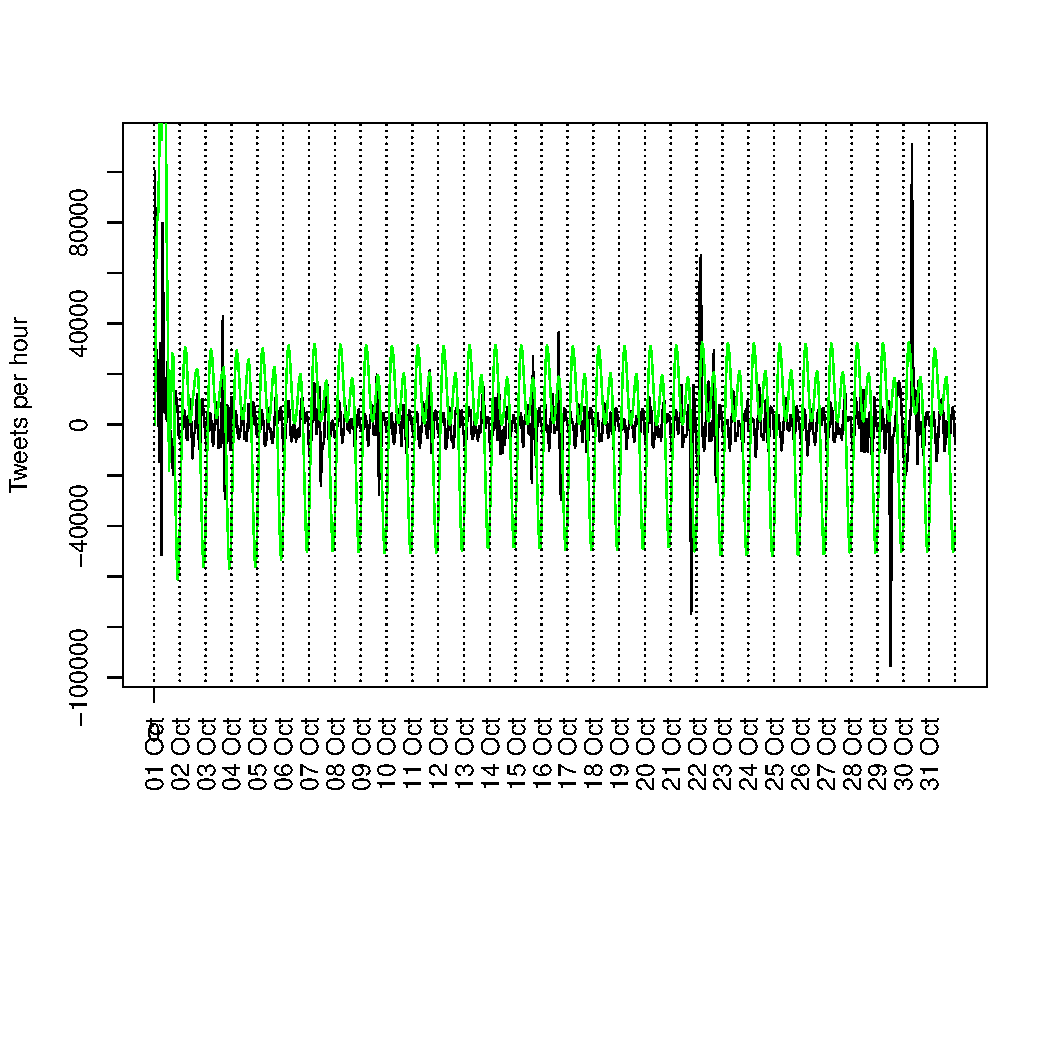
\includegraphics[clip=true,trim=0in 1.5in 0in 1in]
{data-plots_oct/random-walk+days_NUMTWEETS_irregular+repeating.pdf}
\caption{Seasonal and noise components of the volume velocity}
\label{fig:volvel1}
\end{figure}

\begin{figure}
\includegraphics%[clip=true,trim=0in 1.5in 0in 1in]
{data-plots_oct/random-walk+days_NUMTWEETS_level+sma.pdf}
\caption{Stochastic level of the volume velocity}
\label{fig:volvel2}
\end{figure}

\subsection{Sliding window model}

One of the prominent stream processing models is the sliding window model,
where a window of  data  \emph{slides} forwards through the stream. 
The window keeps a fixed amount of history data (fixed in terms of age not size); 
data with a timestamp older that a certain time is removed from the window 
as new data is added. %just created 
The data in the window is processed every time the window slides.
Thus, the sliding window model sets a cut-off age after which
a datapoint has no effect at all on the results of the stream processing algorithm. % of the processing 
This is the simplest way to overcome the problem
that an anomaly in the date, 
such as a burst of tweets about a certain topic,
could affect the mining results more than recent data.
More elaborate methods include dynamically changing the 
sliding window size~\cite{bifet2007learning}, 
smoothing the data~\cite{gilbert2001surfing},
%storing approximate statistics (sketch)
and weighting data according to its age~\cite{giannella2003mining}.

We apply the algorithms to epochs of data, 
similar to the \emph{block evolution} stream mining approach~\cite{ganti2002mining,zhu2003efficient}.
However, our algorithms are not strictly stream processing algorithms.
Stream processing algorithms are supposed to process transactions one at a time
as they arrive, looking at each transaction only once
~--~in other words, they should make one pass on the data then discard it.
This complicates the model of computation % a lot
and there is no justification to process social media data as a stream.
The stream processing model of computation is justified when
the data is not supposed to be stored (such as data from sensor networks),
or when the processing time has to be as short as possible 
such that looking at historic data is an overhead 
(such as in the case of processing stock ticker data, 
where making a decision a few milliseconds 
before/after competitors can translate into profits/losses).
%millions of dollars). 
In the case of social media text, 
the data has to be stored anyway 
and the perception of the human users
makes processing times in the order of seconds %or even minutes
acceptable in a \emph{real time} system.


%We can regard the way we process the social media stream as 
In essence, processing epochs of data is still 
mining a sliding window that is moved forward by time steps of short span.
The time step must be longer than the time needed to mine an epoch of data,
and the performance of our algorithms makes it possible to use a time step
as short as a few seconds for epochs up to a day long.
Figure \ref{fig:runtimeEpochs} shows the runtime of LCM on epochs of
increasing length, and we will show in section \ref{sec:bounding} that our
extensions do not degrade performance.
The times reported in figure \ref{fig:runtimeEpochs} are averages across all
epochs of the specified length in the last 3 months of 2012, % October, November and December,
using a time step that is half the epoch length.
The variance is very low and the confidence bands are not shown because they
appear as dots.  % on top of the bars. 
The \emph{minimum support threshold} used throughout this thesis %, unless otherwise specified,
is 10 occurrences in the hour of day in which the volume velocity is the minimum. % $\alpha=0.0002$.
Figure \ref{fig:avgSupp} shows the average of the actual support threshold to which this minimum support
threshold translates, at different epoch spans.

\begin{figure}
\centering
\scalebox{0.45}{
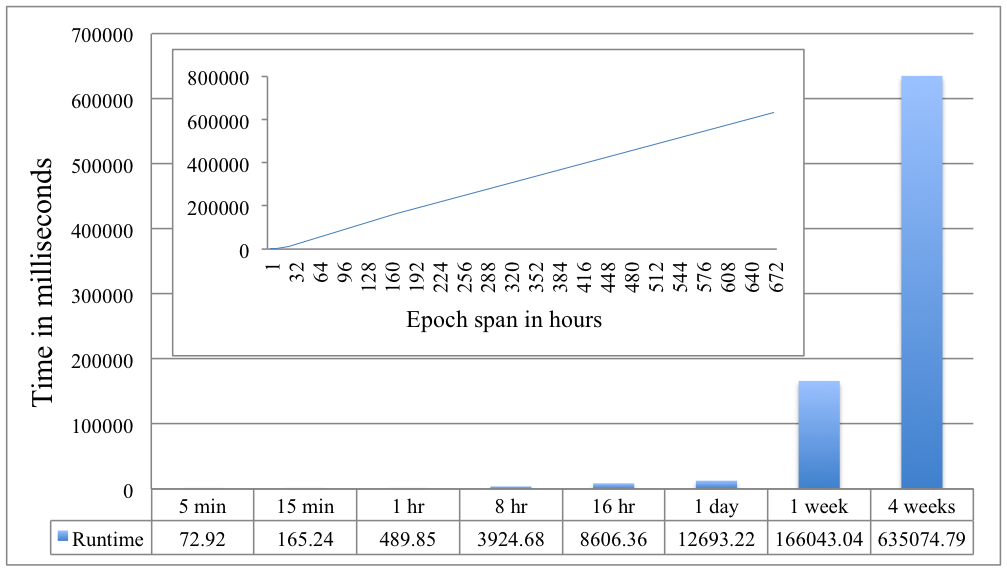
\includegraphics{runtim_epoch-spans_line-over-bars.png}
}
\caption{Mean runtime of LCM at different epoch spans}
\label{fig:runtimeEpochs}
\end{figure}


\begin{figure}
\centering
\scalebox{1}{
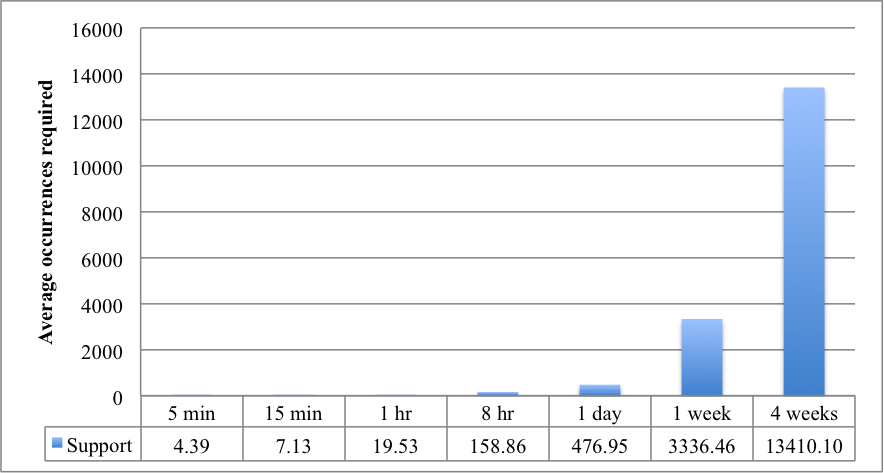
\includegraphics{epochlen_support.png}
}
\caption{Mean support corresponding to minimum support 10, at different epoch spans}
\label{fig:avgSupp}
\end{figure}

%TODONOT elaborate on that.. show figures.
In the rest of this paper we mine epochs of 1 hour span.
The reason behind this choice is an observation that the number of closed
itemsets mined from epochs of span 1 hour or more,
at the same support threshold, remains the same.
This indicates that itemsets mined from shorter epochs of social media text
are not included in the results of mining longer epochs. 
Therefore, the epoch span should be minimized.
However, when the epoch span is shorter than an hour the frequency required
to surpass the support threshold becomes very low,
and number of mined itemsets increases, 
with many noise itemsets appearing in the results.
%Figure \ref{fig:epochLenNumItemsets} shows the number of 
%closed itemsets at different epoch lengthes.. maximal ones too.. but using N-Gram 5.


Regardless of the length of the epoch,
many mined itemsets are combinations of function words.
In the next section, we outline how we reduce the number of itemsets and
eliminate the effect of function words by N-gram filtering.

\section{Filtering Language Constructs}
%\subsection{Tokenizing into Variable Length N-grams}
\label{sec:ngrams}

A large number of itemsets are language constructs that bear no information,
such as ``such as''. 
By treating sequential language constructs, and any other multiword expression,
as one item we eliminate a large number of such itemsets.
We can also eliminate itemsets that are made up of all the different fragments
of the language construct along with other items;
for example, the itemset \{we, did, it, \#teamobama\} can produce 10 other combinations of
length 2 or more.
There are many measures of association that can be used to detect multiword
expressions, but each measure is good only under certain conditions~\cite{ramisch2012broad}.
After preliminary experiments with various measures, we determined that
the best performance
could be obtained by tokenizing the documents into term N-grams with varying N. 


We use term N-gram tokens such that N-grams of high probability are replaced by
(N+1)-grams, resulting in a distribution with no high peaks.  
An N-gram is considered to % of length N
have a high probability if its maximum likelihood estimate
, from a background model,
is higher than a threshold $\eta_N$. 
A background language model built from a long epoch of data 
from the same stream is used for probability estimation.
The language model is simply a hash map of the counts of 
N-grams that appeared within the last month, for N up to 7.

The tokenization of a tweet starts by tokenizing it into unigrams, 
as described in the next section. % \ref{sec:tokenization}.
Then, each
unigram of high probability is replaced by two term bigrams, by
attaching to it the unigrams before and after it.
We keep replacing N-grams of high probability by two (N+1)-grams 
%repeat this for each N $\ge$ 1,for all N-grams
%with probabilities above the threshold 
until there are no more such N-grams. %; thus, the distribution is relatively flat.

The threshold of high probability is different for each value of N. 
The threshold for unigrams is determined as follows: 
We picked a topical term that is known to  steadily  appear with a rather high frequency, 
and is talked about in all languages; `obama'. 
The maximum likely hood estimate of the probability of the term `obama' within the whole collection of Tweets is 0.0001. 
%in a similar fashion to how we determined the support threshold. 
We use $\eta_1 = P(``obama") = 0.0001$.
At each N, the probability threshold is adjusted to account for the increase
in the number of tokens and the overall increase in the grand sum of counts (caused by overlap).
The adjusted $\eta_N$ is:
\begin{equation}\eta_N = \eta_1 \times \frac{\sum_{\{w:\, w \,\in\, W\, and\, w.length \,\le\, N\}}{freq(w)}}{\sum_{\{v:\, v\, \in\, W \,and \,v.length\,=\,1\}}{freq(v)}}\end{equation}


Figure \ref{fig:ngramsLen} shows the effect of increasing the maximum length
of N-grams from 1 to 5 on the number of tokens, the number of closed itemsets,
%of length more than 1, 
and the runtime of mining one hour of data.
The values shown are averages across all one-hour epochs in the month of
November 2012.
The value of $\eta$ used is 0.0001.
Figure \ref{fig:ngramsLen}(a) shows that the number of distinct items
increases substantially as maximum N goes from 1 to 2, then continues increasing
slightly until it starts decreasing at $N \le 5$.
The decrease happens because all 4-grams with probability above the threshold
are parts of tweets from services that use the same text and append a URL,
such as tweets reporting scores from
Game Insight\footnote{http://www.game-insight.com/}.
Such tweets are tokenized into more 4-grams than 5-grams, and the 4-grams
appearing in them do not appear elsewhere.
Thus, each pair is reduced to one 5-gram.
Figure \ref{fig:ngramsLen}(b) shows that the number of itemsets continues to
decrease as expected.
Figure \ref{fig:ngramsLen}(c) shows that runtime also decreases as N goes
from 1 to 5, since LCM runtime is proportional to the number of closed
itemsets, and is not affected by the sparsity of data.
The runtimes in this figure are slightly less than those in
figure \ref{fig:runtimeEpochs} because they do not include the time taken for
writing the posting list of each itemset.

The number of itemsets in the plots include 
itemsets of length 1 (frequent N-grams). 
At $N \le 5$, the number of closed itemsets of length 2 or more
that are mined from an hour epoch averages at 2439.17.
The number of maximal itemsets of length 2 or more
averages at 1831.92.
All of these numbers are counts of distinct unigram sets.
After mining itemsets of term N-grams we flatten the itemsets to sets of unigrams again.
This is necessary since an itemset will have different N-gram set representations,
and its postings list is the union of those of the different representations.
This also removes overlap between N-grams of the same itemset,
making it easier to reason about how itemsets relate to each other.
We will use the relation between an itemset and its subsets to
select interesting itemsets in the next chapter.
%filter out uninformative itemset 


%Notice that the (N+1)-grams replacing an N-gram overlap with each other, with the unigrams that got 
%attached to the N-gram and possibly with other N-grams. 
%However, the  
%We do not prevent overlap, because there is no guarantee that the N-Gram
%created makes any sense.After mining term N-grams we flatten the itemsets to sets of unigrams again.
%This removes overlap between parts of itemsets making it easier to reason
%about how they relate to each other. 
%This is also necessary since an itemset will have different N-gram set
%representations,
%and its postings list is the union of those of the different representations.


\begin{figure}
\centering
\scalebox{0.78}{
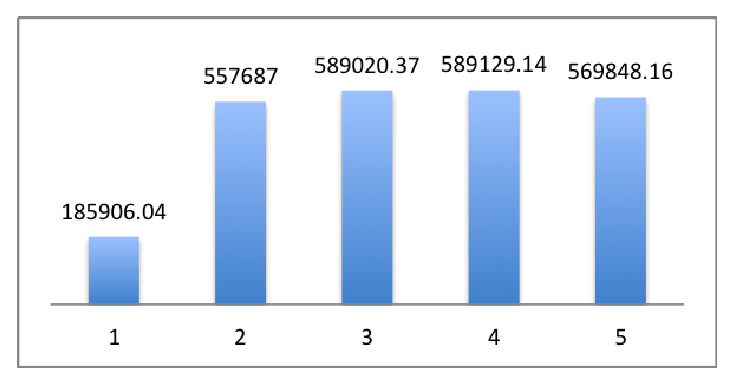
\includegraphics{perf_ngramlen1-5_distinct-items_supp10+_1hr.eps}
}
\\
\begin{tabular}{c}
\\(a) Mean number of distinct items at different values of maximum N \\ \\
\end{tabular}
\\
%\caption{Mean number of distinct items}
%\label{fig:ngramsLenA}
%\end{figure}
%\begin{figure}
%\centering
\scalebox{0.78}{
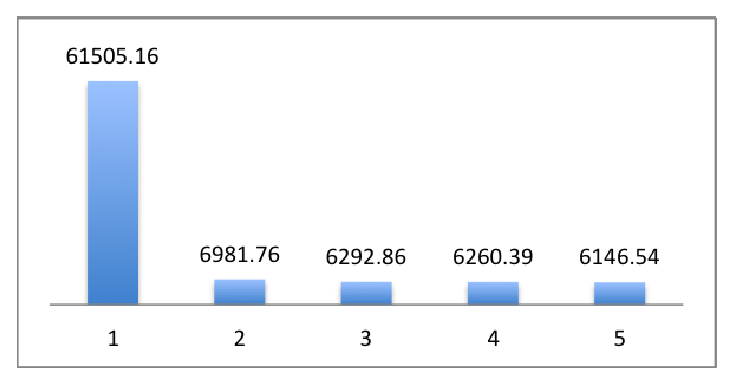
\includegraphics{perf_ngramlen1-5_itemsets_supp10+_1hr.eps}
}
\\
\begin{tabular}{c}
\\(b) Mean number of itemsets at different values of maximum N \\ \\
\end{tabular}
\\
%\caption{Mean number of itemsets}
%\label{fig:ngramsLenB}
%\end{figure}
%\begin{figure}
%\centering
\scalebox{0.78}{
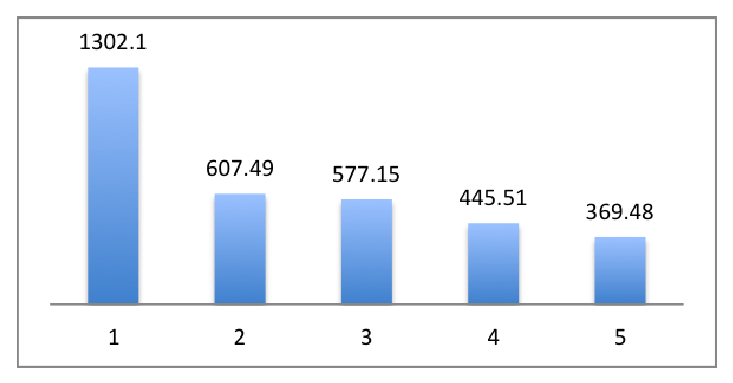
\includegraphics{perf_ngramlen1-5_runtime-millis_supp10+_1hr.eps}
}
\\
\begin{tabular}{c}
\\(c) Mean runtime in milliseconds at different values of maximum N
\end{tabular}
%\caption{Mean runtime in milliseconds}
%\label{fig:ngramsLenC}
\caption{Effect of changing the maximum N-gram length on mining hour long epoches}
\label{fig:ngramsLen}
\end{figure} 

\section{Tokenization}
The data is tokenized into unigrams using white space and punctuation marks as separators. 
The characters `@', `\#' and `\_' are allowed within a unigram, 
while the rest of the punctuation marks are treated as delimiters. % \langle \!\$\%\&()\*\+,.\/:;<=>?[]\^\{|\}\~"`- \rangle .
Only Latin characters  (Unicode code points less than `u024F') and numbers are allowed within a unigram,
and any other characters that are not delimiters are skipped.
The tokenizer also does the following:
\begin{itemize}
\item All URLs are replaced by the token ``URL''. 
\item Runs of the same character is reduced to only 3 repetitions (for example, ``coooool'' is replaced by  ``coool''). 
\item Hashtags are stored twice, with and without the the `\#' character. 
The tag without the `\#' character is left at tag's positions, while the other is appended at the end of the tweet.
This handles cases where the hashtag is used in place of a word, such as ``president \#obama...''.
%\item 
 %All tokens are stored both in their original form, and after applying Lucene's implementation of the Porter stemmer. 
 %We use the original form to select the subset of documents to score, and the stemmed form while scoring. This avoids the disadvantage that stemming retrieves irrelevant documents, while taking advantage of it to count words about the same concept towards the same term frequency. While words sharing the same stem can mean totally different concepts in the context of different documents, it is very likely that they have the same meaning within one document, and this meaning is probably the one desired if the document is retrieved using the unstemmed query term. 
\end{itemize}



% =========================================
% C H A P T E R     4
% =========================================

\chapter{Selecting Interesting Itemsets}
\label{sec:strong}



In section~\ref{sec:ngrams}, we discussed our handling of function words,
using a technique that exploits LCM's tolerance to sparsity.
After applying this technique, the average number of itemsets mined from an
hour of twitter data drops from 61,505 to 6,146.
However, there is still redundancy in the itemsets.


\begin{figure}
\centering
\scalebox{0.5}{
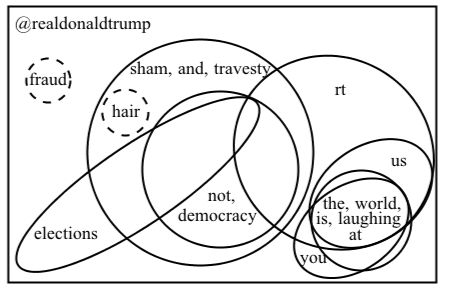
\includegraphics{sham.png}
}
\caption{Closed, distinct and strongly closed sets}
\label{fig:sham}
\end{figure}


The closed property of an itemset is easily violated by modifying one
transaction that contains the itemset and removing one of its items.
While an update operation is not supported in the model of frequent itemsets
mining, a similar effect happens when people are writing about a certain fine
grained topic.
For example, figure \ref{fig:sham} illustrates  itemsets related to Donald
Trump's famous tweets in reaction to Obama's victory in
2012\footnote{http://www.huffingtonpost.com/2012/11/07/donald-trump-election-revolution\_n\_2085864.html}.  
Each area in the figure represents the transactions containing the itemset
formed by concatenating the items in all intersecting ellipses.  

The figure shows the effect of the lack of context and structure in
conversations happening on Twitter.
Because there was originally no way to refer to a certain tweet,
a tweet that sparked a conversation on Twitter had to be quoted in a retweet
along with the retweeter's comment.
This tradition still continues even though tweets can now explicitly reference
one another. 
Due to the 140 characters length limit of tweets the quotation is usually 
edited to be as short as possible by selecting only the most discriminative
words. 

In the figure, the most discriminative words are ``sham, and, travesty''
which are quoted along with Donald Trump's user name in most of the retweets.
Other people choose to also include ``not, democracy'' and/or ``elections'',
and in most of the cases the retweet indicator ``rt'' is added. 
This selection is an act of collaborative filtering,
but it results in many trivially different subsets from the original tweet.
The additions of retweeters also form many different supersets of the of the
original tweet, and some additions represent opinions that are supported
enough to be mined as itemsets. 

To reduce redundancy, we propose two conditions that are not as easily violated 
as the closed condition and use them for selecting itemsets.
The two conditions build on the concept of \emph{association rule confidence}.
Confidence is the basic property used for association rules mining,
and it is used in the definition of $\delta$-free sets~\cite{boulicaut2003free}.
Mining itemsets based on the confidence of rules they induce has long been
recognized as a method for finding
``interesting patterns''~\cite{cohen2001finding},
but since this property is not anti-monotone it cannot be directly used.
%a variation has to be used
%(for example, \emph{all confidence}). % \cite{kim2004ccmine}
The confidence of an assocation rule that the presence of an itemset,
$s_{j}$, implies the presence of another itemset, $s_i$, is  defined as:
\begin{equation}\label{eq:conf}conf(s_j \rightarrow s_i) = \frac{|T_{s_i} \cap T_{s_j}|}{|T_{s_j}|}\end{equation}


\section{Distinct Itemsets}


The \emph{distinct} condition is a novel strengthening of the closed condition
so that it is not violated by trivial differences.
We define a \emph{distinct} itemset as a closed itemset whose frequency
comprises more than a certain proportion of the frequency of its least
frequent subset. 
This condition chooses closed itemsets which substantially violate the closed
condition of their subsets.
The proportion is a parameter, $\kappa$, that controls the selectivity of the
\emph{distinctiveness} condition.
This can be interpreted as selecting itemsets which are implied by a subset
with confidence greater than $\kappa$.
Formally, the set of \emph{distinct} itemsets, $\mathcal{D}$,
is defined as follows:
\begin{equation}\mathcal{D} = \{s: s \in \mathcal{C} \, and \, \exists \; s_{p} \subset s \; where \; \frac{|T_{s}|}{|T_{s_{p}}|} \ge \kappa 
\}\end{equation}

In figure \ref{fig:sham}, \emph{distinct} itemsets are illustrated in solid
lines, and closed itemsets that do not satisfy the distinctiveness condition in dashed lines.
It is clear from the figure that considerable redundancy remains in
\emph{distinct} itemsets.

\section{Strongly Closed Itemsets}
To remove the redundancy in \emph{distinct} itemsets we merge similar ones
into \emph{strongly closed} itemset clusters.
The similarity of a \emph{distinct} itemset,
$s_d$, and another distinct itemset, $s_c$,
is measured as the overlap of the \emph{transactions} containing both of them
with the transactions containing $s_c$. 
A \emph{distinct} itemset is clustered with another itemset if one exists
such that the overlap exceeds a similarity threshold,
which we take to be $1-\kappa$ (the indistinctiveness of $s_d$ from $s_c$).
If more than one satisfies this condition,
the  \emph{distinct} itemset is clustered with the one having the highest
overlap ratio.
When  a \emph{distinct} itemset is clustered with an itemset that is already
part of a cluster, the \emph{distinct} itemset is added to the existing cluster.
Finally, the \emph{strongly closed} itemset is the union of all cluster members,
and its support is the size of the union of their postings lists.
We define the  desired clustering  and the strongly closed itemset
represented by each cluster as follows:
\begin{align*}\label{eq:strongClosedFormal}
\mathcal{R} = \{r: r = \bigcup_i{(s_i, s_j)}\; where\; s_i \in \mathcal{D} \, and \, s_j \in \mathcal{D} 
\\\,and\; \forall_{(s_i,s_j)} \, s_j = \textbf{argmax}_{s_k} conf(s_k \rightarrow s_i) \\\,and \;conf(s_j \rightarrow s_i) \ge (1-\kappa)
\\\, and\;( s_j = r.centroid\; or \; (s_j, r.centroid) \in r )\}
\end{align*}
\begin{equation}S_l = \{w:\, w \in \bigcup_{(s_i, s_j) \in r_l}{s_i} \; where \; r_l \in \mathcal{R}\}\end{equation}

This clustering scheme selects the cluster that contains the itemset which
maximizes the confidence of the rule $conf(s_j \rightarrow s_i)$,
with a lower bound on the overlap to maintain distinctiveness. 
This clustering can be implemented efficiently using techniques similar to
the ones proposed by Bayardo et al. \cite{bayardo2007scaling}.
The main ideas are to limit the comparisons to a few candidates,
and to terminate the comparison early if the similarity threshold will not
be met.
In our case, the postings lists are longer than the itemsets,
so we generate candidates for comparison by calculating similarity between
itemsets.
When calculating the similarity between two postings lists,
we can terminate early if the difference exceeds the maximum difference
permissible to achieve a similarity of $1-\kappa$,
which can be derived from equation \ref{eq:conf}. 

Algorithm~\ref{algo:alliance}  shows a possible implementation.
For each itemset, $s_i$, we find the itemsets produced before it
and overlapping with it in one or more items.
Then we find the candidate, $s_c$, that maximizes
$conf(s_c \rightarrow s_i)$ such that the confidence exceeds $1-\kappa$.
Notice that confidence is not a symmetric measure,
and we only check the confidence of the rule that the clustering candidate
implies the itemset. 


\begin{algorithm}
\SetAlgoLined
\LinesNumbered
\KwIn{$\kappa$: Minimum distinctiveness threshold} 
\KwData{$\mathcal{C}$: Closed itemsets produced by LCM}
\KwResult{$\mathcal{R}$: Strong closed itemset clusters}
\For{$i \gets 2$ to $|\mathcal{C}|$}{
	$C \gets \{s_c: s_c \in \mathcal{C} \, and \, c < i \, and \, |s_c \cap s_i| > 0\}$\;
	$P \gets \{s_p: s_p \in \mathcal{C} \, and \, p < i \, and \, s_p \cap s_i = s_p\}$\;
	$s_p \gets \textbf{argmax}_{s_p \in P}\frac{|T_{s_i}|}{|T_{s_p}|}$ \tcp*{Direct parent}
	\uIf{$\frac{|T_{s_i}|}{|T_{s_p}|} < \kappa$}{continue\tcp*{Not a distinct itemset}}
	$s_m \gets s_i$  \tcp*{Cluster centroid, initially self}
	$maxConf \gets 0$ \tcp*{Best candidate's score}
	\ForEach{$s_c \in C$}{
		$\Delta \gets (1 - (1-\kappa)) |T_{s_c}|$ \tcp*{Maximum difference}
		$\delta \gets$ difference($T_{s_c},T_{s_c \cup s_i},\Delta$) \tcp*{Stops early}
		
		\If{$\delta \le \Delta$}{ 
			$conf \gets \frac{|T_{s_c}| - \delta}{ |T_{s_c}|}$\;
			\If{$conf > maxConf$}{
				$s_m \gets s_k$ \tcp*{Best merge candidate}
				$maxConf \gets conf$ \;
			}
		}
	}
	$\mathcal{R}[s_i] \gets \mathcal{R}[s_m]$ \tcp*{Cluster $s_i$ with $s_m$}
	$\mathcal{R}[s_m].itemset \gets \mathcal{R}[s_m].itemset \cup s_i \cup s_m$\;
	$\mathcal{R}[s_m].postingsList \gets \mathcal{R}[s_m].postingsList \cup s_i.postingsList \cup s_m.postingsList$\;
}
\Return{$\mathcal{R}$}\;
\caption{Forming strongly closed itemset clusters}
\label{algo:alliance}
\end{algorithm}




\section{Temporal Ranking}
\label{sec:rank}

A General Measure of Rule Interestingness
Szymon Jaroszewicz and Dan A. Simovici
University of Massachusetts at Boston

The previous filtering steps reduce the number of itemsets to under 1\% of their
original number.
In this section, we present a method for ranking itemset clusters according to
their novelty when compared to other time periods.
These itemsets can then be presented to users in rank order, providing a
synopis of events in the epoch, or used as input to additional search or
summarization steps.

A good indicator of novelty is the pointwise Kullback-Leibler Divergence (KLD)
between an itemset's probability in the current epoch and in a longer past
epoch~---~the background model.
The KLD of the probability of an itemset $s_i$ in the background
model $Q$ from the current epoch's model $P$ can be considered as
the information gain, IG: 
\begin{align}IG(P(s_i),Q(s_i))  = - (H(P(s_i)) - H(P(s_i),Q(s_i))) \notag\\ = \sum{P(s_i) \log{P(s_i)}} - \sum{P(s_i) \log{Q(s_i)}} \notag\\ = KLD(P(s_i)||Q(s_i))\end{align}

To calculate the collective IG of a strongly closed itemset cluster,
we have to take into account that the itemsets of the cluster are not independent. 
For simplicity we will consider only the pairwise dependence between 
every itemset and the smallest common subset.
%when calculating the IG of the whole cluster.
The joint probability of an itemset, $s_i$, and its superset,
$s_j$, is equal to the probability of the superset.
Thus, the IG of the appearance of an itemset and its superset
together is essentially the IG of the superset.
Also, their pointwise mutual information (PMI) is the self information (SI) of
the subset. Therefore, the IG of a superset is different from the
IG of its subset by the information gained because
of the additional items. 

Hence, the IG of a strongly closed itemset cluster,
$S=\{s_{i1},..,s_{im}\}$, 
can be approximated as the IG of its smallest subset, $s_{min}$,
plus the differences between the IGs of member itemsets and the smallest subset.
We use the squares of the differences, because it can be between two negative number, and we only care about the magnitude of the difference.
To give the self information of the smallest subset the same influence,
we also square it.
Thus, the information gain of a strong closed itemset is given by:
\begin{multline}IG^2(P(s_{i1},...s_{im}),Q(s_{i1},...s_{im})) =\notag\\ I^2(s_{min}) + \notag\\ 
\sum_{j = i1..im}{(IG(P(s_j)||Q(s_j)) - IG(P(s_{min})||Q(s_{min})))^{2}} \end{multline}

The formula above can be used directly for ranking clusters,
but it will favour larger ones.
We normalize by the size of the cluster giving our final ranking formula for
strongly closed itemsets:
\begin{equation}\label{eq:avgIG}\overline{IG}(S) = \frac{IG^2(P(s_{i1},...s_{im}),Q(s_{i1},...s_{im}))}{m}\end{equation}


\chapter{Evaluation}
\label{sec:empirical}


\section{Efficiency}
\label{sec:bounding}
We analyze the performance of the filtering conditions proposed by applying
them to the mining results of all one-hour long epochs in the Twitter data.
The average number of itemsets mined from an hour-long epoch is
2439.17 closed itemsets of length 2 or more;
that is, excluding itemsets that are merely a frequent item.

%The number of length 2 or more maximal itemsets is 1831.92,
%which we provide just as a reference to the result of a basic way of filtering.

Figure \ref{fig:kappa} show the effect of varying $\kappa$ on the mean number
of \emph{distinct} and \emph{strong closed} itemsets.
The number of \emph{distinct} itemsets drops as the distinctiveness threshold
increases.
On the other hand, the number of \emph{strong closed} clusters formed increases
as the similarity (indistinctiveness) threshold decreases.
The dashed line shows that the number of unclustered distinct itemsets reaches
zero at $\kappa=0.5$, explaining why the number of clusters changes very
slightly after that. 
We use $\kappa = 0.25$ in the remainder of the paper,
which is an arbitrary choice based on the definition not the data.
The average number of itemsets (\emph{strongly closed} and unclustered
\emph{distinct}) mined from one-hour epochs at this value of
$\kappa$ is only 224.48, which is about 10\% of the number of closed itemsets.



\begin{figure}

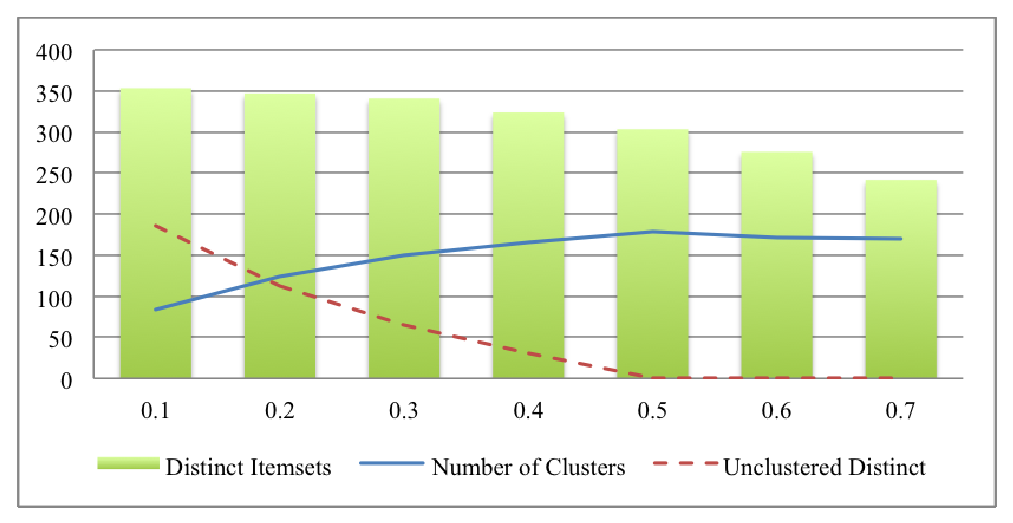
\includegraphics{kappa_effect.eps}
\caption{Effect of changing $\kappa$ on mining results }
\label{fig:kappa}
\end{figure}



Figure \ref{fig:lcmvsfpzhu} shows the total runtime of the LCM algorithm plus
filtering based on the distinct condition and clustering into strong closed
itemsets at different epoch spans.
The runtime of LCM alone is also plotted for reference.
We also plot the performance of another frequent itemset mining algorithm,
FP-Zhu \cite{grahne2004reducing}, which was the runner up at
FIMI 2004~\cite{DBLP:conf/fimi/2004}.
We include it to show that our extensions do not degrade the performance of
LCM even in the context of competitions.
The y-Axis is in logarithmic scale to keep the scale of the plot suitable for
seeing slight differences.
The output of LCM is the input to the filtering and clustering step,
so it is affected by the number of closed itemsets produced.
This explains why it takes slightly longer time for clustering results from
the 15-minute epoch and then takes a constant time for epochs of a longer span. 

The experiments were run using a single threaded Java implementation of
algorithm \ref{algo:alliance}.
The experiments were run on a 1.4GHz processor with 2MB of cache.
Unlike the original LCM algorithm, filtering low confidence itemsets requires
us to keep mined results in memory to calculate the confidence of newly
generated ones.
The memory requirement is not large because the number of itemsets averages
at about 6000.
In our experience with the Twitter data it was enough to keep only a buffer
of 1000 itemsets, and this is what we use for the runtime performance
evaluation and the empirical evaluation of the filtering results in
sections \ref{sec:empirical}.
If all itemsets are kept in memory the runtime increases slightly and
averages at 5.2 seconds for filtering a one-hour epoch.



\begin{figure}
\centering
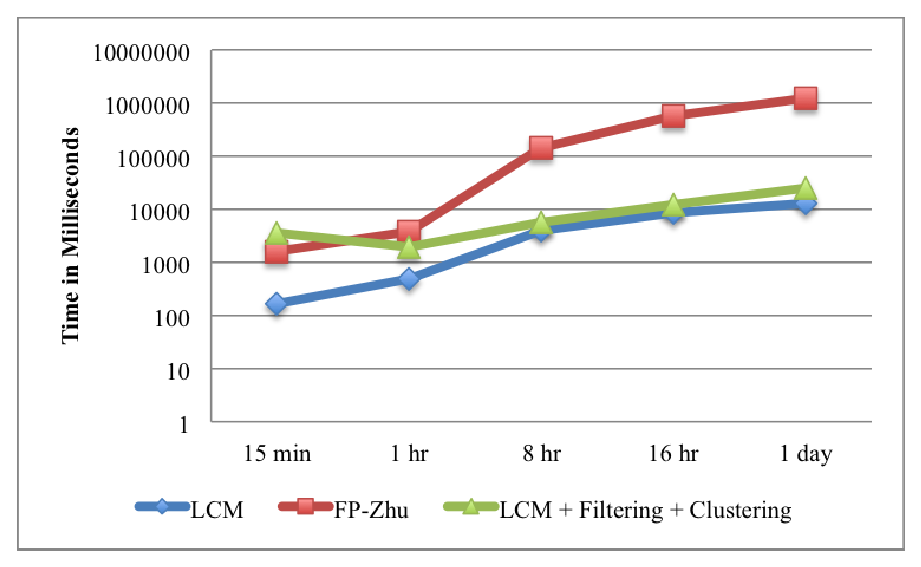
\includegraphics{runtime_lcm-lcm+filter-fpzhu_seconds.eps}
\caption{Runtime of itemset mining alone and with filtering and clustering at different epoch spans}
\label{fig:lcmvsfpzhu}
\end{figure}

\section{Effectiveness}

We now show examples of the performance the proposed methods in creating
a synopses of the 2012 election day, November $6^{th}$, and another less
eventful day, November $9^{th}$.
The background model we use for each day is the results of mining the 4 weeks
before it, using a \emph{minimum support} value of 1 occurrence.
Mining the background model at such a low support increases the number of
produced itemsets, which is desirable for a background model.
All probability estimates are smoothed by add-one smoothing. 

Tables \ref{table:nov6} and \ref{table:nov9}  show the top 3 itemsets for
one-hour epochs in the days examined.
The itemsets shown are the first appearances of the most interesting itemsets;
that is, an hour is shown only if its top 3 feature novel interesting itemsets. The first column is the beginning of the hour, EST time.
The second column is the top itemsets.
The third column is a commentary to explain the itemsets,
but we omit it from table \ref{table:nov9} to save space since the itemsets are self explanatory.

In table \ref{table:nov6}, we can see how the events of the US presidential
elections  unwind from ``get out and vote'' to the projections and debates,
all the way to the ``acceptance speech''.
Early in the day, itemsets about UEFA Champions football matches and a TV show
``Geordie Shore'' appear in the top 3 along with itemsets about the still
uneventful elections.
Actually, the matches keep occupying top positions and timely updates of their
scores appear in the top 30 itemsets, until they end and the elections
heats up.
Shortly after the results of the elections became clear, news that
``weed is legal in Colorado'' occupies the top position.
This exemplifies the power of social media as a collaborative filter,
selecting the news of greatest importance to social media users.
The user centric definition of importance is also evident in attention
given to the ``lady behind Obama  with a flag in her hair'' during the
acceptance speech. 

On November $9^{th}$, table \ref{table:nov9}, the most interesting hour is
15:00.
The MTV Europe Music Awards (MTVEMA) was taking place and votes were solicited
from the audience through Twitter.
This is an example of a topic where people have strongly different opinions.
The top 3 itemsets of the hour 15:00 are supporting ``Katy  Perry'',
``Justin Bieber'' and ``Lady Gaga'' respectively.
They are all reported as separate itemsets, showing how clustering using the
postings lists avoid forming incohesive clusters.
No other major events were happening but many overlapping minor ones happened.
The day started by news about the end of two careers;
the Laker's ``coach Mike Brown'' got fired  and ``CIA director David Petraeus
resigns''.
A personal relationship of Justin Bieber also ends as he
``broke, up, with, Selena, Gomez'' at 22:00.
This event overlaps with his participation in the MTVEMA,
and both topics occupied high (but distinct) rankings. 
By the end of the day in North America, many congratulations for the
Indonesian Hero's day (``Hari Pahlawan'') appear, and the Turkish
commemoration day of Ataturk is also mentioned as the 10th of November has
started in these countries.
These are examples of itemsets from languages with a relatively low number of
users, showing how the absolute popularity of a topic does not affect its rank.
If itemsets from only a specific language is desired,
language identification can be applied on the itemsets and tweets from their
postings lists.
Moving language identification downstream avoids affecting the results of
mining because of error in an upstream component.

\begin{table}

\begin{center}
\small
\def\arraystretch{1.1}
\begin{tabular}{|p{.6cm}|p{2.5cm}|p{5cm}|}

\hline
\multirow{3}{*}{\texttt{13:00}} 	&  0, 1, de, jong 			& De Jong scores for Ajax \\ \cline{2-3} %http://www.dailymail.co.uk/sport/football/article-2228815/Manchester-City-2-Ajax-2--match-report-Siem-Jong-Yaya-Toure-Sergio-Aguero-Champions-League.html
					   	& geordie, shore		& Season 5 of the TV series starts \\ \cline{2-3}
						& get, out, and, vote		& Still early in the U.S. elections day \\\hline

\multirow{3}{*}{\texttt{17:00}} 	&  if, obama, wins		& Speculations regarding elections \\ \cline{2-3}
					   	& USERNAME, spots, my, club		&  Pyramidal marketing scam. Retweeted by people to make money.  \\ \cline{2-3}
						& the, polls, close		& Polls to start closing at 6 PM \\\hline %http://www.huffingtonpost.com/2012/11/06/what-time-do-polls-close_n_2080894.html

\multirow{3}{*}{\texttt{19:00}} 	&  A partir de que idade voc\^{e} considera algu\'{e}m velho?		& Internet meme from Brazil, discussing when to start considering a person old. \\ \cline{2-3}
					   	& food, stamps		& Discussions pertaining to elections \\ \cline{2-3}
						& linda, mcmahon, senate		&  Linda McMahon loses CT senate race \\\hline

\multirow{3}{*}{\texttt{20:00}} 	& obama, got, this		&  Announcing states that Obama got \\ \cline{2-3}
					   	& projected, winner		& Early projections about who will win \\ \cline{2-3}
						& moving, to, canada		&  Reaction to projections \\\hline


\multirow{3}{*}{\texttt{21:00}} 	& elizabeth, warren		&  MA senate elections winner \\ \cline{2-3}
					   	& popular, vote		& Comparing Popular vs Electoral votes \\ \cline{2-3}
						& who, is, the, president?		&  Anticipation for the elections results\\\hline
						

\multirow{3}{*}{\texttt{22:00}} 	& \#forward, \#obama2012		&  Obama won, time to move \#forward \\ \cline{2-3}
					   	& my, president, is, still		& Some were saying Black (skin colour), others Blue (party colour) \\ \cline{2-3}
						& back, in, office		&   Obama is back in office\\\hline

\multirow{3}{*}{\texttt{22:30}} 	& once, you, go, black		& A popular cultural reference.\\ \cline{2-3} %  .. you never go back. 
					   	& @realdonaldtrump, this, elections, ... [his famous tweet] 		& Donald Trump is a Republican and he did not accept Obama's victory. This cluster merges 15 \emph{distinct} itemsets.\\ \cline{2-3}
						& concession, speech, write		&   The losing candidate has to concede before the winner declares victory \\\hline
						
\multirow{3}{*}{\texttt{23:00}} 	& weed, is, legal, in, colorado		&  This piece of news got the attention as soon as it was announced  \\ \cline{2-3}
					   	& karl, rove		& Fox news challenges results from Ohio\\ \cline{2-3}
						& our, country, is, trouble		&   Dramatic reactions to elections \\\hline						
\multirow{3}{*}{\texttt{23:30}} 	& acceptance, speech, wrote		&  Obama wrote his speech, ...\\ \cline{2-3}
					   	& give, his, speech		& ... and is going to deliver it ... \\ \cline{2-3}
						& on, cnn		&   ... on CNN. \\\hline	
						
\multirow{3}{*}{\texttt{00:30}} 	& behind, obama, with, flag, in, her [hair]		&  During the speech, attention on social media goes to a woman appearing behind Obama on TV! \\ \cline{2-3}
					   	& the, best, is, yet, to, come		&  Quote from Obama's speech\\ \cline{2-3}
						& flag, that, weaves	& Play on words about the ``flag in hair'' \\\hline																			
\end{tabular}
\end{center}
\caption{Top 3 itemsets for hours in November 6th}
 \label{table:nov6}
\end{table}

\begin{table}
\begin{center}
\small
\def\arraystretch{1.1}
\begin{tabular}{|p{.6cm}|p{7.5cm}|}

\hline
\multirow{3}{*}{\texttt{12:00}} 
& \#iwillneverunderstand, why\\\cline{2-2}
& breaking, news, head, coach, mike, brown, have, fired  \\\cline{2-2}
& USERNAME, spots, available, my, club \\\hline
\multirow{3}{*}{\texttt{14:00}} 
& cia, director, david, petraeus, resigns \\\cline{2-2}
& voc\^{e}, acha, que \\\cline{2-2}
& \#tvoh [the voice of Holland], babette \\\hline
\multirow{3}{*}{\texttt{15:00}} & \#emawinkaty, i, think, katy, perry, will, be, the, big,  \#mtvema, winner, tweet, your, pick, at, URL
\\ \cline{2-2}
& \#emawinbieber, i, think, justin, bieber, ... [same as above] \\ \cline{2-2}
& \#emawingaga, ... [same as above]  \\\hline														
\multirow{3}{*}{\texttt{22:00}} & justin, bieber, and, selena, gomez, broke, up
\\ \cline{2-2}
& selamat, hari, pahlawan \\\cline{2-2}
& aniyoruz, kemal, mustafa [ataturk] \\ \hline
\end{tabular}
\end{center}
\caption{Top 3 itemsets for hours in November 9th}
 \label{table:nov9}
\end{table}


As a form of comparison, in table \ref{table:mtv} we show the top 3 itemsets picked by the MTV algorithm~\cite{mampaey2011tell} for the same epochs and support.
%for one-hour epochs. 
% 
We show hours in which the top 3 itemsets included interesting itemsets. For brevity, we truncate itemsets that are complete tweets and append the tweet id for reference.
% 
%It is noteworthy that tweets that spark a conversation contribute multiple redundant itemsets, and several of them are ranked high.
% (Nov. 6 22:00). This stresses the importance of clustering.
%The harm from redundancy is amplified by the low values of K that has to be used. 
% to attain an acceptable runtime.
The input to the algorithm was transactions made up of N-grams up to 5 terms long, which helped the algorithm converge faster since the distribution is flatter. 
The use of N-grams also overcomes the dominance of language constructs, which are otherwise ranked high in all hours. 
All the topically relevant itemsets chosen by MTV are present in the top 50 \emph{strongly closed itemsets}.

 
 \begin{table}
 \begin{center}
\small
\def\arraystretch{1.1}
\begin{tabular}{|p{.6cm}|p{7.5cm}|}

\hline

\texttt{Nov}
& @realdonaldtrump,this,elections,...[266035509162303492] \\\cline{2-2} %This election is a total sham and a travesty. We are not a democracy! 
\texttt{6th,}
&we, re, all, in, this, together, ..., bo [266031109979131904]  \\\cline{2-2} % That's how we campaigned, and that's who we are. Thank you. -bo
\texttt{22:00} & @realdonaldtrump,our,country,is,...[266037143628038144] \\\hline %Our country is now in serious and unprecedented trouble...like never before.




\texttt{Nov}
&URL,and,autotweet,checked,followed,me,today,unfollowed \\\cline{2-2}
\texttt{6th,}
&house,of,representatives,shouldnt,...[266040877552656385]  \\\cline{2-2} % House of Representatives shouldn't give anything to Obama unless he terminates Obamacare.
\texttt{23:00} & URL,\#android,\#androidgames,\#gameinsight \\\hline 


\texttt{Nov}
&URL,and,autotweet,checked,followed,me,today,unfollowed \\\cline{2-2}
\texttt{6th,}
&URL,\#android,\#androidgames,\#gameinsight  \\\cline{2-2} 
\texttt{23:30} &@barackobama,@ryanseacrest, what, was, your, first, words, in, reaction, to, re, election, 2\\\hline 


\texttt{Nov}
&URL,and,autotweet,checked,followed,me,today,unfollowed \\\cline{2-2}
\texttt{6th,}
&the, best, is, yet, to, come \\\cline{2-2} 
\texttt{00:00} & URL,\#android,\#androidgames,\#gameinsight \\\hline 



\texttt{Nov}
& \#emawinbieber, i, think, justin, bieber, ... [see table \ref{table:nov9}] \\\cline{2-2}
\texttt{9th,}
&@boyquotations,do,everyone,follow,followers,gain,more \\\cline{2-2} 
\texttt{15:00} & \#emawinkaty, i, think, katy, perry, ... [see table \ref{table:nov9}] \\\hline 
\end{tabular}
\end{center}
\caption{Top 3 picked by the MTV algorithm}
 \label{table:mtv}
\end{table}

 

\chapter{Conclusion and future work}
\label{sec:concfut}
We have proposed a method for efficiently creating temporal synposes of social
media streams, based on a frequent itemset mining algorithm that is suitable
for sparse data, LCM.
Our method summarizes an hour of Twitter data (116920 tweets on average) into
224 itemsets in 1945.68 milliseconds on average,
and scales for longer epochs of data.
The direct application of LCM on one-hour epochs of Twitter data results in
an average of 61505.16 closed itemsets and takes 2506.58 milliseconds on
average.
The improvement is due to the following contributions: 
(1) strengthening  the closure condition such that it selects an itemset only if
it is distinctively different from its subsets and other itemsets, and 
(2) using variable length N-grams to mitigate the effect
of the skewness of the frequency distribution of unigrams.
The distinctiveness between two itemsets is based on a parameter, $\kappa$, which controls tolerance to redundancy. %Even though the use or variable length N-grams

Another important contribution is a method for ranking itemsets based on their temporal novelty.
The top 3 itemsets from the hours of election day and another less eventful
day shows that the synopses captures important events, and might reasonably
be directly presented to users as a summary.
A possible future direction is to use itemsets that appear as a sequence for
building extractive coherent summaries of the social media stream at
different times.

We aim to exploit the synopses for temporal query expansion in our future work. Terms from itemsets relevant to a query (or occurring in a relevant document)
can be used for query expansion, thus acting as precomputed results of 
pseudo-revelance feedback.
We also wish to explore ways to make use of the temporal signal during mining,
such as when calculating similarity during clustering.

 
%----------------------------------------------------------------------
% END MATERIAL
%----------------------------------------------------------------------

% B I B L I O G R A P H Y
% -----------------------

% The following statement selects the style to use for references.  It controls the sort order of the entries in the bibliography and also the formatting for the in-text labels.
\bibliographystyle{plain}
% This specifies the location of the file containing the bibliographic information.  
% It assumes you're using BibTeX (if not, why not?).
\cleardoublepage % This is needed if the book class is used, to place the anchor in the correct page,
                 % because the bibliography will start on its own page.
                 % Use \clearpage instead if the document class uses the "oneside" argument
\phantomsection  % With hyperref package, enables hyperlinking from the table of contents to bibliography             
% The following statement causes the title "References" to be used for the bibliography section:
\renewcommand*{\bibname}{References}

% Add the References to the Table of Contents
\addcontentsline{toc}{chapter}{\textbf{References}}

\bibliography{yaboulna-uwaterloo_mmath-thesis}
% Tip 5: You can create multiple .bib files to organize your references. 
% Just list them all in the \bibliogaphy command, separated by commas (no spaces).

% The following statement causes the specified references to be added to the bibliography% even if they were not 
% cited in the text. The asterisk is a wildcard that causes all entries in the bibliographic database to be included (optional).
\nocite{*}

\end{document}

